\pdfoutput=1
% Options for packages loaded elsewhere
\PassOptionsToPackage{unicode}{hyperref}
\PassOptionsToPackage{hyphens}{url}
\PassOptionsToPackage{dvipsnames,svgnames,x11names}{xcolor}
\documentclass[
  11pt,
]{article}
\usepackage{xcolor}
\usepackage[margin=1in]{geometry}
\usepackage{amsmath,amssymb}
\setcounter{secnumdepth}{5}
\usepackage{iftex}
\ifPDFTeX
  \usepackage[T1]{fontenc}
  \usepackage[utf8]{inputenc}
  \usepackage{textcomp} % provide euro and other symbols
\else % if luatex or xetex
  \usepackage{unicode-math} % this also loads fontspec
  \defaultfontfeatures{Scale=MatchLowercase}
  \defaultfontfeatures[\rmfamily]{Ligatures=TeX,Scale=1}
\fi
\usepackage{lmodern}
\ifPDFTeX\else
  % xetex/luatex font selection
\fi
% Use upquote if available, for straight quotes in verbatim environments
\IfFileExists{upquote.sty}{\usepackage{upquote}}{}
\IfFileExists{microtype.sty}{% use microtype if available
  \usepackage[]{microtype}
  \UseMicrotypeSet[protrusion]{basicmath} % disable protrusion for tt fonts
}{}
\makeatletter
\@ifundefined{KOMAClassName}{% if non-KOMA class
  \IfFileExists{parskip.sty}{%
    \usepackage{parskip}
  }{% else
    \setlength{\parindent}{0pt}
    \setlength{\parskip}{6pt plus 2pt minus 1pt}}
}{% if KOMA class
  \KOMAoptions{parskip=half}}
\makeatother
\usepackage{longtable,booktabs,array}
\usepackage{caption}
\captionsetup[table]{skip=6pt}
\newcounter{none} % for unnumbered tables
\usepackage{calc} % for calculating minipage widths
% Correct order of tables after \paragraph or \subparagraph
\usepackage{etoolbox}
\makeatletter
\patchcmd\longtable{\par}{\if@noskipsec\mbox{}\fi\par}{}{}
\makeatother
% Allow footnotes in longtable head/foot
\IfFileExists{footnotehyper.sty}{\usepackage{footnotehyper}}{\usepackage{footnote}}
\makesavenoteenv{longtable}
\setlength{\emergencystretch}{3em} % prevent overfull lines
\providecommand{\tightlist}{%
  \setlength{\itemsep}{0pt}\setlength{\parskip}{0pt}}

\usepackage[T1]{fontenc}
\usepackage{newtxtext,newtxmath}
\usepackage{amsmath,amssymb}
\usepackage{booktabs}
\usepackage{graphicx}
\usepackage{etoolbox}
\usepackage{caption}
\captionsetup{font=small,labelfont=bf,justification=justified}
\AtBeginEnvironment{longtable}{\small}
\AtBeginEnvironment{tabular}{\small}
\setlength{\emergencystretch}{3em}
\renewcommand{\arraystretch}{1.15}
\usepackage{microtype}
\usepackage{needspace}
\AtBeginEnvironment{longtable}{\needspace{20\baselineskip}}
\usepackage{bookmark}
\IfFileExists{xurl.sty}{\usepackage{xurl}}{} % add URL line breaks if available
\urlstyle{same}
% fallback for those not using the hyperref driver hyperxmp:
\makeatletter
\@ifundefined{xmpquote}{\newcommand{\xmpquote}[1]{#1}}{}
\makeatother
\hypersetup{
  pdftitle={Bounding cross-trial temporal coupling in a loophole-free Bell test},
  colorlinks=true,
  linkcolor={black},
  filecolor={Maroon},
  citecolor={Blue},
  urlcolor={[rgb]{0.1,0.25,0.5}},
  pdfcreator={LaTeX via pandoc}}

\title{Bounding cross-trial temporal coupling in a loophole-free Bell
test}
\author{Christos Georgitzikis\\
\normalsize Independent Researcher}
\date{5 September 2026}

\begin{document}
\maketitle
\begin{abstract}
Bell's theorem admits one loophole that no experiment can close in
principle: measurement independence. Retrocausal and time-symmetric
models exploit this opening, but the class of models in which the click
probability at one trial depends on measurement settings at \emph{other}
trials has been formalised theoretically but never given an experimental
bound. We bound it on public raw records from the CURBy
device-independent randomness beacon --- ten pulses of
\(1.5 \times 10^{7}\) trials each, spanning twenty-two months, analysed
separately and never spliced.

The result that depends on no model is a bound in bits. Scanning every
lag \(|k| \le 10{,}000\) between one party's outcome and the other
party's setting,

I(O ; S at lag k) \textless{} \(1.13 \times 10^{-6}\) bits per trial,

at family-wise \(\alpha\) = 0.05 (Bonferroni, 40,002 hypotheses). This
is 1/362 of the same-trial outcome--setting information measured on the
same records, and the outcome--outcome information at nonzero lag is
bounded below 1/13,384 of the Bell correlation at k = 0. As a guessing
advantage, no outcome lets an adversary predict any other trial's
setting with a bias above \(1.25 \times 10^{-3}\).

Translated into the parameters of an explicit model --- a click
probability shifted by a kernel-weighted sum of other trials' settings,
with kernel width \(\tau\) and coupling strength \(\varepsilon\) --- the
same data exclude \(\varepsilon\) above \(7.6 \times 10^{-2}\) at
\(\tau\) = 1 trial and \(4.4 \times 10^{-4}\) at \(\tau\) = \(10^{4}\)
trials on a single pulse, for symmetric, future-only, past-only and
one-sided exponential kernels: 208 tests, zero detections. This map is
model-dependent by construction; it is the bound above re-expressed in
the units of one model class, and within the tested class the
sensitivity follows an approximately universal 1/\(\sqrt{Q}\) scaling
with \(Q=\sum_k W(k)^2\), the rigorous exclusion being stated for the
four explicit families. Combining the ten pulses by inverse-variance
weights, with the pulses shown to be uncorrelated, the excluded coupling
falls to \(1.9 \times 10^{-2}\) and \(1.2 \times 10^{-4}\) at the same
two widths: the strongest statement these data support, quoted alongside
the single-pulse map rather than in its place.

The absence of cross-trial memory that device-independent randomness and
DI-QKD assume is thereby checked empirically on an operating beacon, at
the stated sensitivity. The result is null. Its value is that the region
is now mapped rather than assumed empty.
\end{abstract}

\section{Introduction}

Bell's theorem rests on locality, realism, and measurement independence
--- the assumption that the settings chosen by the experimenters are
statistically independent of whatever variables determine the outcomes.
Loophole-free experiments {[}1,2,3{]} have closed the locality and
detection loopholes. Measurement independence cannot be closed by
experiment even in principle, since any test of it must presuppose that
some choices are free {[}4,8{]}.

It can nevertheless be \emph{bounded}, and bounding it is not a
philosophical exercise. Hall {[}4{]} showed that only a small relaxation
of measurement independence suffices for a local model to reproduce
quantum correlations, which makes the permitted size of the relaxation a
physically meaningful quantity. Retrocausal programmes {[}5,6,7{]}
remain the principal route to a local account of Bell correlations, and
are unexcluded by any experiment to date.

Two quantities must be kept apart. Hall's measure {[}4{]} is
\(I(X,Y:\Lambda)\), the mutual information between the settings and the
hidden variable, and it admits no experimental upper bound in a standard
Bell test {[}8{]}: \(\Lambda\) is by construction unobservable, and a
model may place arbitrary correlation there. What we bound is \(I(O;S)\)
at nonzero lag, between two recorded quantities.

The two are related by the data-processing inequality in one direction
only. Since the outcome is generated from \(\lambda\),
\(I(O(i);S(i+k)) \le I(\lambda(i);S(i+k))\); a small observed value does
not force a small hidden one. The converse fails, and we do not claim
it. The bound constrains models by their observable consequences, which
is the only handle an experiment has, and is sufficient for the purpose:
measurement dependence that produces no observable signature in the
measured outcome statistics is not constrained by this analysis.

The retrocausal models cited above are almost exclusively
\emph{within-trial}: the outcome depends on the setting of the same
measurement, chosen slightly later in time. This note addresses a
different class --- models in which the dependence extends \emph{across}
trials, so that the click probability at trial \emph{i} is influenced by
settings at trials \(i \pm k\). Such models predict a directly
observable signature: nonzero mutual information between an outcome and
a setting separated in the trial sequence.

In the standard taxonomy of loopholes {[}25{]} the assumption at issue
here is neither locality nor detection but the freedom-of-choice
assumption, and specifically its cross-trial part: not whether a setting
is correlated with the hidden variable of its own trial, but whether it
is correlated with the outcome of another.

We are not aware of a direct experimental test of this class. The
nearest neighbours are the memory loophole {[}10{]}, where cross-trial
dependence is admitted and handled by adversarially valid statistics
rather than measured, and the theoretical treatment of measurement
dependence across runs by Pope and Kay {[}14{]}, which supplies no
experimental limit. Published bounds on measurement dependence --- the
measurement-dependent locality parameter of Pütz et al.~{[}15{]},
bounded experimentally by Aktas et al.~{[}16{]}, and the
spacetime-region bounds of the cosmic Bell tests {[}17,18{]} --- are
within-trial and in a different parametrisation, and are not directly
comparable to \(\varepsilon\). No published limit known to us constrains
outcome--setting correlation as a function of trial separation.

Santos {[}26{]} asks a related question about the same physical effect
and answers the opposite half of it. He shows that memory effects in
photon-pair experiments cannot produce a loophole large enough to rescue
local hidden variables --- a statement about what memory could
\emph{accomplish}. What follows is a measurement of how much of it is
\emph{there}. Neither implies the other: a device could carry
cross-trial memory far too weak to fake a Bell violation and still leak
more than a protocol assuming none would tolerate. It is that quantity,
at every separation up to ten thousand trials, that is measured here.

The nearest currency to ours is the one measured in bits. Barrett and
Gisin {[}22{]} showed that if Bob's choices are completely free, every
correlation obtainable from projective measurements on a singlet can be
reproduced by a local model in which the mutual information between
Alice's choice and the local variables is at most one bit --- so a bound
in bits on setting--variable correlation is the natural currency for how
much measurement dependence a model needs. Hall and Branciard {[}23{]}
sharpened the accounting in the CHSH scenario, finding that an optimal
causal model needs about 0.080 bits of such information to reproduce the
maximal quantum violation while a retrocausal one, in which later
settings influence earlier source variables, needs about 0.046. Koh et
al.~{[}24{]} carried the same relaxation into device-independent
randomness expansion and bounded what an adversary gains from it. All
three quantify information involving the hidden variable, at a single
trial; the bound below is on information between two recorded
quantities, at a separation in trials, and the data-processing
inequality relates the two in one direction only (above). It cannot be
compared with them numerically, and we do not.

\section{The model class}

\textbf{Notation.} A \emph{trial} is one entry of the beacon record. A
\emph{pulse} is one beacon round; the two words are used interchangeably
below and rounds are identified by their beacon index. For trial
\emph{i}, \(S_A(i), S_B(i) \in \{1,2\}\) are the two parties' setting
choices and \(O_A(i), O_B(i) \in \{0,1\}\) are their outcomes, 1 =
detector click. Where the party is immaterial we write S and O. For the
coupling term settings are encoded as \(S(i)\in\{-1,+1\}\). The symbol
\emph{k} always denotes a lag in trials, never a count. The symbol
\(\lambda\) denotes the hidden variable of the models under discussion;
it is never a measured quantity in this work.

Measurement independence in its usual form asserts that the click
probability at trial \emph{i} is independent of all settings other than
the local one at that trial. We relax this in a specific, parametrised
way. Writing \(p(i)\) for the click probability at trial \emph{i}:

\begin{equation}
p(i) \;=\; p_0\!\left(S_{\mathrm{own}}(i)\right) \;+\; \alpha\,\varepsilon \sum_k W_\tau(k)\, S_{\mathrm{other}}(i+k)
\label{eq:model}
\end{equation}

Here \(p_{0}\)(\(S_{\mathrm{own}}\)) is the ordinary same-trial click
probability given the party's own setting --- standard quantum
mechanics, measured directly --- and \(W_{\tau}\) is a kernel of
characteristic width \(\tau\) normalised to max W = 1. Two parameters
carry the physics:

\begin{itemize}
\tightlist
\item
  \textbf{\(\varepsilon\)} --- coupling strength. We adopt the
  normalisation \(\varepsilon\) = 1 \(\equiv\) as strong as the ordinary
  quantum-mechanical same-trial connection, so that \(\varepsilon\) is
  directly interpretable as a fraction of standard physics. This is a
  convention, not a physical statement. The factor \(\alpha\) that
  implements it is defined in \S3.
\item
  \textbf{\(\tau\)} --- temporal extent, in trials. This is the
  parameter that gives the scan range physical meaning: without it, the
  choice of \(|k| \le 10{,}000\) would be arbitrary. \S4.1 converts
  trials to seconds.
\end{itemize}

The scan range itself is not arbitrary either. Statistically it is
almost free: a lag k is estimated from n \(-\) \textbar k\textbar{}
trials, so at the edge of the window the sample is still 99.93\% of the
total and the loss of power is 0.03\%; the sample would shrink by 10\%
only near \textbar k\textbar{} \(\approx 1.5 \times 10^{6}\), where the
loss of power would still be just 5\%. In physical units the window is
not a single number: at the instrument's nominal rate of about 250,000
trials per second (\S4.1) it spans \(\approx\) 40 ms, and the metadata
bound of 51 \(\mu\)s per trial puts it at \(\le\) 510 ms. Only the
shorter end can be assumed, so the coverage claim is made against 40 ms:
electronic and fast mechanical correlation times of a table-top optical
apparatus fall inside it, and anything slower --- thermal drift of an
optical table, which lives on seconds to minutes --- does not. Slower
mechanisms are not thereby unconstrained; they would appear as drift
common to whole pulses rather than as structure in k, and are addressed
by the setting-correlation test of \S5.1 and by the ten-pulse comparison
of \S6.4, which spans twenty-two months.

Equation (1) is a linearisation, and holds while the perturbation is
small against the baseline rate. Since the settings are independent and
equiprobable, the injected term has standard deviation
\(\alpha\varepsilon\sqrt{Q}\) across trials, so the condition is
\(\alpha\varepsilon\sqrt{Q} \ll p_0\). The largest value of
\(\alpha\varepsilon\sqrt{Q}\) anywhere on the single-pulse map occurs
for the past-only kernel at \(\tau\) = 1 in the channel
\(O_{\mathrm{B}}\) vs \(S_{\mathrm{A}}\), where
\(\varepsilon_{\mathrm{excl}}\) = \(1.382 \times 10^{-1}\) and Q =
0.386; with \(\alpha_{\mathrm{B}}\) = \(1.8283 \times 10^{-3}\) this is
\(1.570 \times 10^{-4}\), or 2.3\% of that channel's \(p_{0}\) =
\(6.87087 \times 10^{-3}\). Everywhere else it is smaller. The model is
therefore used only in the regime where its linear form is accurate.

\subsection{Why cross-trial coupling is a class worth testing}

The model above is not introduced arbitrarily. Two established lines of
work define hidden-variable classes with exactly this structure, and
neither has been given an experimental bound as a function of
separation.

\textbf{The memory loophole.} Barrett, Collins, Hardy, Kent and Popescu
{[}10{]} observed that in a repeated Bell experiment the hidden
variables of one trial may depend on the settings and outcomes of
\emph{previous} trials, since a real source and real detectors carry
state between runs; the same reuse of stateful devices is what makes
memory attacks possible in device-independent cryptography {[}19{]}. The
loophole is normally addressed statistically, by deriving p-values valid
without the i.i.d. assumption {[}11,12,13{]}. That approach establishes
that a violation remains significant under adversarial memory; it does
not measure how much memory is actually present. The present work asks
the complementary question: given the data, how large could such a
dependence be?

\textbf{Measurement dependence across runs.} Pope and Kay {[}14{]}
formalised limited measurement dependence in multiple runs of a Bell
test, treating the settings of one run as partially determined by
variables shared with others. Their treatment is theoretical; it
supplies no experimental limit. Our \(\varepsilon\) is a direct
operational analogue of the quantity their framework leaves
unconstrained.

Beyond these, three mechanisms would produce the signature we search
for:

\begin{enumerate}
\def\labelenumi{\arabic{enumi}.}
\item
  \emph{Source memory.} A hidden variable retaining state across trials
  couples \(\lambda(i)\) to conditions at neighbouring trials, including
  the settings applied there. The natural kernel width \(\tau\) is then
  the correlation time of the source state in units of trials.
\item
  \emph{Non-Markovian environment.} If the two wings share an
  environment with memory, the effective hidden variable at trial
  \emph{i} is a functional of a window of the environment's history
  rather than of its instantaneous state.
\item
  \emph{Temporally extended boundary conditions.} Retrocausal accounts
  {[}5,6,7{]} fix the hidden variable using a future boundary condition,
  and it matters what that condition is a condition \emph{on}. In the
  terminology of {[}6{]} the settings are inputs to the model and the
  outcomes are outputs; such models are better called future-input
  dependent, and what they give up is \(\lambda\)-independence --- the
  requirement that the distribution of \(\lambda\) be independent of the
  settings a and b that lie in its future. The future-dependence is
  therefore on the \emph{setting}, a parameter fixed from outside the
  model. The outcome is not a second future condition; it is the thing
  the model is built to explain. What the scan of \S3 measures is
  exactly the first quantity: \(\delta(k)\) is the dependence of an
  outcome at trial \emph{i} on the \emph{setting} at trial \emph{i+k}.
  Outcome--outcome dependence is a different object, bounded separately
  in \S6.5, and is not what a future-input dependent account calls for.

  Such accounts are normally posed within a single trial, the relevant
  future input being the setting of the same measurement, and the
  condition is then imposed on an instantaneous hypersurface. That last
  step is the fragile one. In the two-boundary field models the weight
  from which probabilities are built is a flux integral of the field's
  four-current over a \emph{closed} hypersurface in spacetime {[}20{]},
  and restricting that surface to two parallel instants is presented as
  a special case to be relaxed rather than as a requirement {[}21{]}. A
  duration enters those models explicitly: the predictions depend on the
  interval \(t_{0}\) between the two boundaries, they depart from
  standard quantum mechanics if either boundary constrains the energy
  --- a conserved quantity --- to a precision near \(\hbar/t_0\), and
  two measurements cannot be placed in a well-defined order at a
  separation shorter than the time a measurement itself takes {[}20{]}.

  Our own reading of this, offered as an observation and not as anyone's
  stated position, is that the durationless instant is the part that
  does not survive. A future condition posed physically is carried by
  something that persists over an interval, so the ``moment of
  measurement'' acquires a finite extent, and a constraint of finite
  extent reaches neighbouring trials. \(\tau\) is that extent, in units
  of trials, and the future-only kernels of \S2.2 are its natural form.

  The formalisation of this picture remains open. We know of no model
  that derives a cross-trial kernel W(k) from a two-boundary or
  future-input dependent starting point, and we do not supply one. The
  bound does not require it: the only property of the kernel that enters
  the exclusion is \(Q(\tau)=\sum_k W(k)^2\) (\S2.2, \S6.3), so whatever
  form the formalisation takes, its coupling is bounded by the tables of
  \S6.3 as soon as its W is evaluated on the same lag grid.
\end{enumerate}

A fourth possibility is mundane and worth stating, because the test
excludes it too: correlated drift between the setting generators and the
detector state would produce cross-trial outcome--setting correlation
with no new physics whatsoever. A null result is therefore also a
systematics check on the experiment, independent of any interpretation.

\textbf{What is bounded is a rate, not a hidden variable.} We model the
click probability p(i), an observable, and bound the mutual information
between two observables. This is deliberate and is the reason the bound
exists at all. A dependence residing entirely in an unobservable
\(\lambda\), leaving no trace in the outcome statistics, is not
constrained here --- but neither does it do any work: a measurement
dependence that never reaches the outcomes cannot help a local model
reproduce quantum correlations. What we bound is the operationally
effective part.

\subsection{Kernels}

Four kernels are considered. In every one of them the lag k = 0 is
excluded: \(W_{\tau}\)(0) = 0 by definition. The k = 0 term would be the
dependence of an outcome on the setting of the \emph{same} trial --- the
no-signalling condition, a different physical question from cross-trial
coupling, already tested separately in the ``Cross-pair I at k = 0'' row
of Table 3 (\S5). A model class named cross-trial must not contain the
within-trial term, and the matched filter of \S6.3 must not integrate
over it. Every kernel, Q, and filter in this paper is therefore
evaluated over 0 \textless{} \(|k| \le 10{,}000\).\footnote{An earlier
  version of this analysis included k = 0 in the symmetric kernel.
  Removing it changes the symmetric bounds at small \(\tau\) only --- by
  a factor of 1.7 at \(\tau\) = 1, 3--7\% at \(\tau\) = 10, about 1\% at
  \(\tau\) = 100 and below 0.5\% for \(\tau \ge\) 1,000 --- and leaves
  the one-sided kernels, which never contained k = 0, unchanged.}

The quantity

\begin{equation}
Q(\tau) \;=\; \sum_{0<|k|\le 10{,}000} W_\tau(k)^2
\label{eq:Q}
\end{equation}

is the only property of the kernel that enters the final bound (\S6.3),
so it is tabulated here alongside each shape:

\begin{longtable}[]{@{}
  >{\raggedright\arraybackslash}p{(\linewidth - 6\tabcolsep) * \real{0.2500}}
  >{\raggedright\arraybackslash}p{(\linewidth - 6\tabcolsep) * \real{0.2500}}
  >{\raggedright\arraybackslash}p{(\linewidth - 6\tabcolsep) * \real{0.2500}}
  >{\raggedright\arraybackslash}p{(\linewidth - 6\tabcolsep) * \real{0.2500}}@{}}
\caption{The four kernel shapes and their Q relative to the symmetric
kernel.}\tabularnewline
\toprule\noalign{}
\begin{minipage}[b]{\linewidth}\raggedright
Kernel
\end{minipage} & \begin{minipage}[b]{\linewidth}\raggedright
W(k)
\end{minipage} & \begin{minipage}[b]{\linewidth}\raggedright
\(Q(\tau)\)/\(Q_{\mathrm{sym}}\), \(\tau \ge\) 10
\end{minipage} & \begin{minipage}[b]{\linewidth}\raggedright
at \(\tau\) = 1
\end{minipage} \\
\midrule\noalign{}
\endfirsthead
\toprule\noalign{}
\begin{minipage}[b]{\linewidth}\raggedright
Kernel
\end{minipage} & \begin{minipage}[b]{\linewidth}\raggedright
W(k)
\end{minipage} & \begin{minipage}[b]{\linewidth}\raggedright
\(Q(\tau)\)/\(Q_{\mathrm{sym}}\), \(\tau \ge\) 10
\end{minipage} & \begin{minipage}[b]{\linewidth}\raggedright
at \(\tau\) = 1
\end{minipage} \\
\midrule\noalign{}
\endhead
\bottomrule\noalign{}
\endlastfoot
symmetric & exp(\(- k^{2}\)/2\(\tau^{2}\)), all \(k\) \(\ne\) 0 & 1 &
1 \\
future-only & exp(\(- k^{2}\)/2\(\tau^{2}\)) for \(k>0\), else 0 & 0.500
& 0.500 \\
past-only & exp(\(- k^{2}\)/2\(\tau^{2}\)) for \(k<0\), else 0 & 0.500 &
0.500 \\
exponential future & exp(\(-\)k/\(\tau\)) for \(k>0\), else 0 &
\(\approx\) 0.28 & 0.203 \\
\end{longtable}

With k = 0 absent from all four, the one-sided Gaussians carry exactly
half the symmetric Q at every \(\tau\), to machine precision. The
exponential ratio is not a constant: for \(\tau \gtrsim\) 10 it lies
between 0.270 and 0.289 (0.270 at \(\tau\) = 10, 0.281 at \(\tau\) =
100, 0.282 at \(\tau\) = 1,000, 0.289 at \(\tau\) = \(10^{4}\), where
the window truncates the two kernels differently), which is why the
column is given as \(\approx\) 0.28. Q is computed exactly as a finite
sum over the scan window, never asymptotically; the symmetric kernel has
Q = 0.773 at \(\tau\) = 1 and 2.545 at \(\tau\) = 2. One detail of the
discrete lag grid: since k = 0 is excluded, every kernel peaks at k =
\(\pm 1,\) where W is exp(\(-1\)/2\(\tau^{2}\)) or exp(\(-1\)/\(\tau\))
rather than exactly 1 --- 0.61 and 0.37 at \(\tau\) = 1, within 1\% of 1
for \(\tau \ge\) 10. The analysis uses these W as written. At small
\(\tau\) the quoted \(\varepsilon\) is therefore expressed in units of
this sub-unity peak; restated in strictly peak-normalised units the
excluded coupling would be \emph{smaller} by the same factor, so the
tables err on the conservative side.

The one-sided kernels matter because retrocausal models are future-input
dependent {[}6{]} and therefore asymmetric; a symmetric-only analysis
would leave the natural case untested. The sign convention is
\(k>0 \equiv\) future: the setting at trial i+k influences the outcome
at trial i.

A consequence of excluding k = 0 deserves note. None of the four filters
touches the single lag that carries genuine quantum correlation and
known systematics; the nearest lags, k = \(\pm 1,\) are where detector
deadtime would appear, and Table 3 shows it does not at this sample
size. What the filters integrate is cross-trial structure only.

\section{Observable signature}

Write \(p_{0}\) for the baseline click probability and \(\delta(k)\) for
half the difference in click rate between the two settings at lag k. The
model of \S2 gives

\begin{equation}
\delta(k) \;=\; \alpha\,\varepsilon\,W_\tau(k)
\label{eq:delta}
\end{equation}

where \(\alpha\) is the device sensitivity. For small \(\delta\),
standard expansion of the mutual information about independence yields

\begin{equation}
I(k) \;\approx\; \frac{\delta(k)^2}{2\ln 2\; p_0(1-p_0)} \;=\; C\,\varepsilon^2 W_\tau(k)^2, \qquad C = \frac{\alpha^2}{2\ln 2\; p_0(1-p_0)}
\label{eq:mi}
\end{equation}

For the Gaussian kernel this is a bell curve of width \(\tau/\sqrt2\) in
\(I\) and \(\tau\) in \(\delta\).

Here \(p_{0}\) is the \emph{marginal} click probability of the
\(2\times2\) table, \(p_0=(c_1+c_2)/n\) with \(c_s\) the click count
under setting s and n the number of trials --- not an average taken as
an approximation. Because the settings are balanced 50/50 this coincides
with \((r_1+r_2)/2\) to within \(4.9 \times 10^{-5}\) relative, the
residual being \((m_1-m_2)(r_1-r_2)/2n\) with \(m_s\) the number of
trials under setting s and \(r_s = c_s/m_s\). The marginal is the
expansion point at which the second-order form is exact to leading
order; the alternative choices \(r_{1}\), \(r_{2}\), or
\(\sqrt{r_1r_2}\) would give ratios of 1.37, 0.77, and 1.03 against the
measured value, whereas the marginal gives 0.986.

\textbf{Calibration.} \(\alpha\) is not a free parameter. It is fixed by
the measured same-pair lag-0 dependence, which is ordinary quantum
mechanics. On round 28297 the two settings give click rates \(r_{1}\) =
\(4.96662 \times 10^{-3}\) and \(r_{2}\) = \(8.89072 \times 10^{-3}\),
hence \(\delta\)(0) = \(1.96206 \times 10^{-3} \pm 2.14 \times 10^{-5}\)
and \(\alpha\) = \(1.9621 \times 10^{-3} \pm\) 1.1\%. The same
construction on Bob's wing gives \(r_{1}\) = \(5.04249 \times 10^{-3}\),
\(r_{2}\) = \(8.69908 \times 10^{-3}\) and \(\alpha_{\mathrm{B}}\) =
\(1.8283 \times 10^{-3}\), with marginal click probabilities \(p_{0}\) =
\(6.92833 \times 10^{-3}\) for Alice and \(6.87087 \times 10^{-3}\) for
Bob. Both are needed: the map is computed per channel, and every
quantity quoted for \(O_{\mathrm{B}}\) vs \(S_{\mathrm{A}}\) --- the
dashed curves of Figure 3, the joint bounds of Table 7, and the worst
point of the map --- uses \(\alpha_{\mathrm{B}}\), not
\(\alpha_{\mathrm{A}}\).

The second-order approximation reproduces the exactly computed mutual
information to 1.35\% (\(4.036 \times 10^{-4}\) against
\(4.091 \times 10^{-4}\), the latter from the four-term \(p\log p\) sum
with no expansion). The relevant small parameter is not \(p_{0}\) but
\(\delta\)/\(p_{0}\) = 0.28. The prediction is low, hence conservative.
This gives C = \(4.036 \times 10^{-4}\) bits per trial per
\(\varepsilon^{2}\).

\textbf{The exclusion map does not use this approximation.} The bound of
\S6.3 is built from \(\hat\varepsilon=T/(\alpha Q)\) with
\(T=\sum_k W(k)\hat\delta(k)\) from measured click rates,
\(\alpha=\delta(0)=(r_2-r_1)/2\), and \(Q=\sum_k W(k)^2\) purely
geometric. None of these contains \(p_{0}\) or any expansion.
Reconstructing the map from these raw quantities and comparing against
the published values at 208 points gives a maximum relative difference
of \(2.2 \times 10^{-16}\). The approximation enters only the
model-independent bound of \S6.1 and the translation constant C.

The two settings differ in click rate by a factor 1.79, an intentional
asymmetry of the Eberhard configuration {[}9{]}. The resulting large
\(\alpha\) works in our favour: since
\(\varepsilon_{\mathrm{excl}} \propto 1/\alpha\), a device sensitive to
its settings yields a tight bound on \(\varepsilon\).

\textbf{Verification.} The derivation was tested rather than assumed.
Synthetic coupling of known (\(\varepsilon\), \(\tau\)) was injected
into the real data --- real settings retained, so that the true setting
autocorrelation is preserved --- and the resulting \(I(k)\) compared
against prediction. Across \(\tau\) = 1, 10, 100, 1000 and three
\(\varepsilon\) each, mean ratios were 1.012 (\(\delta\) amplitude),
1.002 (\(\delta\) width), and 1.005 (I width against the predicted
\(\tau/\sqrt2\)), the fits taken over k \(\ne\) 0 since the kernel has
no k = 0 term (\S2.2). An \(\varepsilon\) = 0 control was run before
each \(\tau\) and produced a flat curve in every case. Injected
probabilities are clipped to {[}0,1{]}; a point is declared invalid if
more than 0.1\% of trials clip, and the \(\varepsilon\) of each
injection is chosen automatically to stay below that limit. The observed
clipping never exceeded 0.026\%.

\section{Data}

The CURBy beacon {[}3{]} publishes per-trial records from a
loophole-free Bell test at NIST: settings and outcomes for both parties,
in acquisition order, prior to randomness extraction. Each pulse
contains \(1.5 \times 10^{7}\) trials after the protocol stopping
criterion.

Ten pulses were analysed: five consecutive (rounds 28293--28297,
spanning 65 minutes on 2025-08-22) and five spread across the archive
(rounds 1000, 15000, 22000, 23000, 26000; 2023-10-31 to 2025-06-28). The
full span is twenty-two months. These are reported separately, since
pulses from different dates necessarily differ in derived calibration
parameters. The protocol configuration is identical across all ten,
verified over 25 rounds spanning the archive. The click rate falls from
0.93\% (round 1000) to 0.64\% (round 26000), with the 2025 pulses at
0.69\%: the apparatus changed materially across the interval sampled.

Exact download URLs, byte counts and SHA-256 digests for every round
used are recorded in \texttt{results/curby\_manifest.json} of the code
repository, so the input can be verified bit for bit.

\subsection{Trials to seconds --- an upper bound only}

The beacon metadata contains no per-trial timing field. What it does
contain is stage timestamps (\texttt{request} \(\rightarrow\)
\texttt{precommit} \(\rightarrow\) \texttt{randomness}). The interval
\texttt{request -> precommit} covers acquisition \emph{plus} unknown
overhead, so it yields an \textbf{upper bound}: for round 28297, 774.34
s over 15,190,485 recorded trials, i.e.~\textbf{\(\le\) 51.0 \(\mu\)s
per trial}. On that bound \(\tau\) = 1 is \(\le\) 51 \(\mu\)s and
\(\tau\) = 10,000 is \(\le\) 510 ms.

This is not a constant of the dataset. For the ten pulses analysed here:

\begin{longtable}[]{@{}
  >{\raggedright\arraybackslash}p{(\linewidth - 8\tabcolsep) * \real{0.2000}}
  >{\raggedright\arraybackslash}p{(\linewidth - 8\tabcolsep) * \real{0.2000}}
  >{\raggedright\arraybackslash}p{(\linewidth - 8\tabcolsep) * \real{0.2000}}
  >{\raggedright\arraybackslash}p{(\linewidth - 8\tabcolsep) * \real{0.2000}}
  >{\raggedright\arraybackslash}p{(\linewidth - 8\tabcolsep) * \real{0.2000}}@{}}
\caption{Upper bound on the time per trial, for each analysed pulse. The
record count is constant to 0.3\%; the acquisition interval is
not.}\tabularnewline
\toprule\noalign{}
\begin{minipage}[b]{\linewidth}\raggedright
Round
\end{minipage} & \begin{minipage}[b]{\linewidth}\raggedright
Date
\end{minipage} & \begin{minipage}[b]{\linewidth}\raggedright
request \(\rightarrow\) precommit
\end{minipage} & \begin{minipage}[b]{\linewidth}\raggedright
Records
\end{minipage} & \begin{minipage}[b]{\linewidth}\raggedright
\(\mu\)s per trial (upper bound)
\end{minipage} \\
\midrule\noalign{}
\endfirsthead
\toprule\noalign{}
\begin{minipage}[b]{\linewidth}\raggedright
Round
\end{minipage} & \begin{minipage}[b]{\linewidth}\raggedright
Date
\end{minipage} & \begin{minipage}[b]{\linewidth}\raggedright
request \(\rightarrow\) precommit
\end{minipage} & \begin{minipage}[b]{\linewidth}\raggedright
Records
\end{minipage} & \begin{minipage}[b]{\linewidth}\raggedright
\(\mu\)s per trial (upper bound)
\end{minipage} \\
\midrule\noalign{}
\endhead
\bottomrule\noalign{}
\endlastfoot
1000 & 2023-10-31 & 168.4 s & 15,228,817 & 11.1 \\
15000 & 2024-03-07 & 350.9 s & 15,227,680 & 23.0 \\
22000 & 2024-07-17 & 483.3 s & 15,223,405 & 31.7 \\
23000 & 2025-05-13 & 510.5 s & 15,182,270 & 33.6 \\
26000 & 2025-06-28 & 598.7 s & 15,191,281 & 39.4 \\
28293 & 2025-08-22 & 641.4 s & 15,191,016 & 42.2 \\
28294 & 2025-08-22 & 647.0 s & 15,182,571 & 42.6 \\
28295 & 2025-08-22 & 679.4 s & 15,186,766 & 44.7 \\
28296 & 2025-08-22 & 730.7 s & 15,190,447 & 48.1 \\
28297 & 2025-08-22 & 774.3 s & 15,190,485 & 51.0 \\
\end{longtable}

The bound grows by a factor of 4.6 in twenty-two months at constant
record count, for reasons the metadata does not explain. The published
description of the instrument {[}3{]} states a nominal rate --- ``about
250,000 trials every second'', with 15 million trials acquired in
\(\approx 60\) s --- for the same protocol configuration analysed here
(the 15,000,000-trial stopping criterion). At that nominal rate one
trial is \(\approx 4\) \(\mu\)s, \(\tau\) = 1 is \(\approx 4\) \(\mu\)s
and \(\tau\) = 10,000 is \(\approx 40\) ms, and the request
\(\rightarrow\) precommit interval is dominated by overhead rather than
acquisition, which would also account for its growth across the archive.
The nominal figure is quoted alongside the metadata bound, not in place
of it: it is the only per-trial timing the records themselves support,
and the nominal rate is not verifiable from the records. \textbf{The
\(\tau\) axis is therefore reported in trials throughout. The conversion
above applies to round 28297 only, is an upper bound rather than a
measurement, and must not be transferred to other rounds.}

\section{Validation}

No result was accepted before the following passed. Significance for
mutual-information quantities is quoted throughout as
\textbf{\(\sqrt{G}\)}, where \(G = 2n\ln 2\cdot I\) is asymptotically
\(\chi^2(1)\) for a \(2\times2\) table (\S6.1). Two entries use the
Eberhard statistic instead and are marked: there the scale is
J/\(\sigma_{\mathrm{J}}\), defined in \S6.2.

\begin{longtable}[]{@{}
  >{\raggedright\arraybackslash}p{(\linewidth - 4\tabcolsep) * \real{0.3333}}
  >{\raggedright\arraybackslash}p{(\linewidth - 4\tabcolsep) * \real{0.3333}}
  >{\raggedright\arraybackslash}p{(\linewidth - 4\tabcolsep) * \real{0.3333}}@{}}
\caption{Validation checks passed before any result was
accepted.}\tabularnewline
\toprule\noalign{}
\begin{minipage}[b]{\linewidth}\raggedright
Check
\end{minipage} & \begin{minipage}[b]{\linewidth}\raggedright
Expected
\end{minipage} & \begin{minipage}[b]{\linewidth}\raggedright
Observed
\end{minipage} \\
\midrule\noalign{}
\endfirsthead
\toprule\noalign{}
\begin{minipage}[b]{\linewidth}\raggedright
Check
\end{minipage} & \begin{minipage}[b]{\linewidth}\raggedright
Expected
\end{minipage} & \begin{minipage}[b]{\linewidth}\raggedright
Observed
\end{minipage} \\
\midrule\noalign{}
\endhead
\bottomrule\noalign{}
\endlastfoot
Eberhard J at k = 0 & violation & +11.7 to +18.8
(J/\(\sigma_{\mathrm{J}}\)), all ten pulses \\
Same-pair I at k = 0 & large & \(4.091 \times 10^{-4}\) bits, G = 8,508
\(\rightarrow\) \textbf{92.2\(\sigma\) (\(\sqrt{G}\))} \\
Cross-pair I at k = 0 & zero (no-signalling) & \(2.14 \times 10^{-8}\)
bits (0.67\(\sigma\)) and \(2.09 \times 10^{-11}\) bits
(0.02\(\sigma\)) \\
Shift sign & injected k = +3 recovered at k = +3 & +134.2
(J/\(\sigma_{\mathrm{J}}\)) at k = +3, on synthetic data \\
Detector deadtime & visible at \textbar k\textbar{} = 1, absent beyond &
\textbf{2.7\(\sigma\) (\(\sqrt{G}\)) at k = \(-1\) in \(O_{\mathrm{B}}\)
vs \(S_{\mathrm{B}}\) --- observed but not significant} \\
Mirror filter & one-sided filters distinguish direction & correct filter
+10, mirrored 1.56 \\
Setting independence & zero at every lag & max 4.83\(\sigma\) over
20,001 lags, 0 above threshold (\S5.1) \\
Pulse independence & \(\hat\delta(k)\) uncorrelated between pulses & max
\textbar r\textbar{} = 0.018 over 90 pulse pairs (2.6\(\sigma\)), 0
above 3\(\sigma\) (\S6.4) \\
Oscillatory coupling & no periodic structure in \(\hat\delta(k)\) & 0 of
200,000 frequencies above threshold, ten pulses (\S6.8) \\
\end{longtable}

The deadtime row is a negative finding and is reported as such. The
largest effect at k = \(-1\) anywhere in round 28297 is 2.7\(\sigma\)
(\(\sqrt{G}\)) in Bob's same-pair channel; Bob's cross-pair channel
gives 2.4\(\sigma\) and both of Alice's channels give below
0.6\(\sigma\). All are far below the 4.85\(\sigma\) threshold of \S6.1,
so the experiment does \emph{not} resolve detector deadtime at this
sample size, and the argument for instrument sensitivity rests on the
same-trial correlation (362\(\times\) the bound) and the Bell
correlation (13,384\(\times\) the bound) instead. An earlier draft
quoted ``+6.2\(\sigma\)'' for this row; that figure came from a
100-shuffle empirical null whose standard deviation was 25\% below the
\(\chi^2(1)\) value, on a different significance scale, and is
withdrawn.

The shift-sign test is not decorative: an error of sign would exchange
``future'' and ``past'', inverting the question. The mirror-filter test
establishes that the one-sided filters are genuinely directional rather
than symmetric filters in disguise.

Three implementation errors were found and corrected during development:
a bit extraction returning \{0,3\} rather than \{0,1\}; a block-reversal
permutation producing out-of-range indices for lengths that are not
powers of two; and an invalid null comparing biased data against
unbiased surrogates. Each would have invalidated everything downstream.
They are reported here because the credibility of a null result rests
entirely on the auditing that produced it.

\subsection{Correlated settings would fake the signal}

One mechanism would produce exactly the signature we search for without
any new physics, and it must be excluded before the bound means
anything. Alice's outcome depends strongly on Alice's \emph{own} setting
--- that is ordinary quantum mechanics, and it is the large effect this
analysis calibrates against, \(\delta_A = 1.96\times10^{-3}\). If Bob's
setting at trial i+k were correlated with Alice's at trial i, the
cross-pair channel would show a signal built entirely from that one
dependence.

The size is fixed by the algebra. With settings encoded as \(\pm 1\) and
equiprobable,
\(\mathbb{E}[O_A \,|\, S_B(i+k)=s] = p_0 + \delta_A\,\rho(k)\,s\) with
\(\rho(k) = \mathrm{Corr}(S_A(i), S_B(i+k))\), so

\begin{equation}
\delta_{\mathrm{phantom}}(k) \;=\; \delta_A\,\rho(k)
\label{eq:phantom}
\end{equation}

and, passed through the same matched filter, the fake coupling is

\begin{equation}
\varepsilon_{\mathrm{phantom}}(\tau) \;=\; \frac{1}{Q(\tau)}\sum_k W_\tau(k)\,\rho(k)
\label{eq:phantom-eps}
\end{equation}

in which \(\alpha\) cancels: the phantom \(\varepsilon\) is just the
kernel-weighted mean of the setting correlation, directly comparable
with \(\varepsilon_{\mathrm{excl}}\).

Measuring \(\rho(k)\) for every \(|k| \le 10{,}000\) by FFT:

\begin{longtable}[]{@{}
  >{\raggedright\arraybackslash}p{(\linewidth - 8\tabcolsep) * \real{0.2000}}
  >{\raggedright\arraybackslash}p{(\linewidth - 8\tabcolsep) * \real{0.2000}}
  >{\raggedright\arraybackslash}p{(\linewidth - 8\tabcolsep) * \real{0.2000}}
  >{\raggedright\arraybackslash}p{(\linewidth - 8\tabcolsep) * \real{0.2000}}
  >{\raggedright\arraybackslash}p{(\linewidth - 8\tabcolsep) * \real{0.2000}}@{}}
\caption{Correlation between the two setting sequences, and each
sequence with itself, across the full lag range. The standard error is
\(1/\sqrt{n} = 2.58\times10^{-4}\), evaluated at the analysed sample of
n = 15,000,000 trials --- the stopping-criterion cut described in the
footnote of \S6.1. At the full record count of the file, 15,190,485, it
would be \(2.566 \times 10^{-4}\), 0.6\% smaller.}\tabularnewline
\toprule\noalign{}
\begin{minipage}[b]{\linewidth}\raggedright
Correlation
\end{minipage} & \begin{minipage}[b]{\linewidth}\raggedright
max \textbar{}\(\rho\)\textbar{}
\end{minipage} & \begin{minipage}[b]{\linewidth}\raggedright
at lag
\end{minipage} & \begin{minipage}[b]{\linewidth}\raggedright
in units of \(1/\sqrt{n}\)
\end{minipage} & \begin{minipage}[b]{\linewidth}\raggedright
above threshold
\end{minipage} \\
\midrule\noalign{}
\endfirsthead
\toprule\noalign{}
\begin{minipage}[b]{\linewidth}\raggedright
Correlation
\end{minipage} & \begin{minipage}[b]{\linewidth}\raggedright
max \textbar{}\(\rho\)\textbar{}
\end{minipage} & \begin{minipage}[b]{\linewidth}\raggedright
at lag
\end{minipage} & \begin{minipage}[b]{\linewidth}\raggedright
in units of \(1/\sqrt{n}\)
\end{minipage} & \begin{minipage}[b]{\linewidth}\raggedright
above threshold
\end{minipage} \\
\midrule\noalign{}
\endhead
\bottomrule\noalign{}
\endlastfoot
\(\mathrm{Corr}(S_A(i), S_B(i+k))\) & \(1.246 \times 10^{-3}\) &
\(-9,438\) & 4.83\(\sigma\) & 0 / 20,001 \\
\(\mathrm{Corr}(S_A(i), S_A(i+k))\), \(k \ne 0\) &
\(9.683 \times 10^{-4}\) & \(-635\) & 3.75\(\sigma\) & 0 / 20,001 \\
\(\mathrm{Corr}(S_B(i), S_B(i+k))\), \(k \ne 0\) &
\(1.104 \times 10^{-3}\) & +9,301 & 4.28\(\sigma\) & 0 / 20,001 \\
\end{longtable}

Nothing reaches the 4.848\(\sigma\) threshold, and the same conclusion
follows from the mutual information of the settings computed with the
machinery and threshold of \S6.1: max \(I(S_A(i) ; S_B(i+k))\) =
\(1.121 \times 10^{-6}\) bits per trial at the same lag, G = 23.29
against a threshold of 23.50, 0 of 20,001 above.

The largest point deserves its own sentence, because it is the closest
call in this work. Across the 20,001 lags the standardised correlations
are textbook normal --- mean \(-0.004,\) standard deviation 1.005,
Kolmogorov--Smirnov p = 0.86, 62 lags above 3\(\sigma\) against 54
expected --- and the 4.83\(\sigma\) point at lag \(-9,438\) is isolated,
its immediate neighbours being 1.15, 0.14, \(-0.24\) and
\(-0.27 \sigma\). Its family-corrected p-value is 0.027: a one-in-forty
fluctuation among twenty thousand, which is what a Bonferroni threshold
exists to absorb. It is also at a lag unrelated to anything in the
outcome analysis.

Taken at face value regardless, the phantom signal is far below the
sensitivity. The largest \(\delta_{\mathrm{phantom}}\) is
\(2.45 \times 10^{-6}\), which is 0.11 of the statistical error on
\(\hat\delta\) at a single lag (\(2.14 \times 10^{-5}\)). Through the
matched filter, across all four kernels and all 26 values of \(\tau\),
\(\varepsilon_{\mathrm{phantom}}\) never exceeds 0.0073 of
\(\varepsilon_{\mathrm{excl}}\): \textbf{the fake signal is at least 138
times below the single-pulse bound at every point of the map}.

\textbf{All ten pulses.} Since the headline result is the joint bound of
\S6.4, a correlated pair of generators in \emph{any} pulse would
contaminate it. The same test was therefore run on all ten:

\begin{longtable}[]{@{}
  >{\raggedright\arraybackslash}p{(\linewidth - 8\tabcolsep) * \real{0.2000}}
  >{\raggedright\arraybackslash}p{(\linewidth - 8\tabcolsep) * \real{0.2000}}
  >{\raggedright\arraybackslash}p{(\linewidth - 8\tabcolsep) * \real{0.2000}}
  >{\raggedright\arraybackslash}p{(\linewidth - 8\tabcolsep) * \real{0.2000}}
  >{\raggedright\arraybackslash}p{(\linewidth - 8\tabcolsep) * \real{0.2000}}@{}}
\caption{Setting cross-correlation in each of the ten pulses. Nothing
anywhere reaches the threshold, by correlation or by mutual
information.}\tabularnewline
\toprule\noalign{}
\begin{minipage}[b]{\linewidth}\raggedright
Round
\end{minipage} & \begin{minipage}[b]{\linewidth}\raggedright
max \textbar{}\(\rho\)\textbar{}
\end{minipage} & \begin{minipage}[b]{\linewidth}\raggedright
at lag
\end{minipage} & \begin{minipage}[b]{\linewidth}\raggedright
in units of \(1/\sqrt{n}\)
\end{minipage} & \begin{minipage}[b]{\linewidth}\raggedright
above threshold
\end{minipage} \\
\midrule\noalign{}
\endfirsthead
\toprule\noalign{}
\begin{minipage}[b]{\linewidth}\raggedright
Round
\end{minipage} & \begin{minipage}[b]{\linewidth}\raggedright
max \textbar{}\(\rho\)\textbar{}
\end{minipage} & \begin{minipage}[b]{\linewidth}\raggedright
at lag
\end{minipage} & \begin{minipage}[b]{\linewidth}\raggedright
in units of \(1/\sqrt{n}\)
\end{minipage} & \begin{minipage}[b]{\linewidth}\raggedright
above threshold
\end{minipage} \\
\midrule\noalign{}
\endhead
\bottomrule\noalign{}
\endlastfoot
1000 & \(9.761 \times 10^{-4}\) & +4,532 & 3.78\(\sigma\) & 0 /
20,001 \\
15000 & \(1.144 \times 10^{-3}\) & +1,277 & 4.43\(\sigma\) & 0 /
20,001 \\
22000 & \(1.176 \times 10^{-3}\) & +2,137 & 4.56\(\sigma\) & 0 /
20,001 \\
23000 & \(1.085 \times 10^{-3}\) & \(-2,286\) & 4.20\(\sigma\) & 0 /
20,001 \\
26000 & \(1.088 \times 10^{-3}\) & +1,106 & 4.21\(\sigma\) & 0 /
20,001 \\
28293 & \(1.077 \times 10^{-3}\) & \(-4,930\) & 4.17\(\sigma\) & 0 /
20,001 \\
28294 & \(1.230 \times 10^{-3}\) & +9,968 & 4.76\(\sigma\) & 0 /
20,001 \\
28295 & \(1.029 \times 10^{-3}\) & +9,439 & 3.98\(\sigma\) & 0 /
20,001 \\
28296 & \(1.096 \times 10^{-3}\) & +8,518 & 4.25\(\sigma\) & 0 /
20,001 \\
28297 & \(1.246 \times 10^{-3}\) & \(-9,438\) & 4.83\(\sigma\) & 0 /
20,001 \\
\end{longtable}

Nothing in any pulse reaches the threshold, on either statistic: 0 of
200,010 tests by correlation and 0 of 200,010 by mutual information.
Seen across the whole set, the 4.83\(\sigma\) point discussed above also
loses its edge of interest: the expected largest \textbar z\textbar{}
among 200,010 standard normals is 4.56, so observing 4.83 has a
family-corrected p of 0.24. It is the ordinary maximum of a large
sample, not a feature.

Against the joint bound the phantom is correspondingly small. Taking the
worst single pulse against the joint bound gives a ratio of 0.039;
propagating the phantom into the joint estimate with the same
inverse-variance weights as the data gives 0.015. \textbf{The fake
signal is at least 65 times below the joint bound at every point of the
map.} Setting independence, to the precision the data allow, is not an
assumption here but a measurement --- in every pulse used.

\section{Results}

\subsection{Model-independent bound}

Full scan of round 28297, 20,001 lags per pair, 40,002 hypotheses in
total. The empirical Bonferroni threshold is impractical at this
multiplicity (it would require \textasciitilde{}\(8 \times 10^{5}\)
shuffles), so we use the analytic result that \(G = 2n\ln 2\cdot I\) is
asymptotically \(\chi^2(1)\) for a \(2\times2\) table. This was
calibrated against 2,000 real shuffles per pair before use: mean G =
0.988 and 0.995 against 1.000 predicted, KS p = 0.59 and 0.69.

\textbf{Confidence level.} All bounds in this paper are stated at
family-wise \(\alpha\) = 0.05 with a Bonferroni correction over 40,002
hypotheses, i.e.~per-test p = \(1.25 \times 10^{-6}\), equivalently
\(z > 4.848\) on the \(\sqrt{G}\) scale. The corresponding
mutual-information threshold is \(1.130 \times 10^{-6}\) bits per
trial.\footnote{All statistics in this paper are computed on exactly the
  first 15,000,000 records of each pulse --- the protocol stopping
  criterion, the same cut the beacon's own extraction pipeline applies.
  The raw files carry 15,182,270 to 15,228,817 records (\S4.1), so
  1.20\% to 1.50\% of each pulse is discarded. Evaluated at the full
  15,190,485 records of round 28297, the threshold would be
  \(1.116 \times 10^{-6}\) bits per trial, 1.3\% lower; truncation can
  only cost sensitivity, so the stated numbers are conservative.}

\begin{longtable}[]{@{}
  >{\raggedright\arraybackslash}p{(\linewidth - 8\tabcolsep) * \real{0.2000}}
  >{\raggedright\arraybackslash}p{(\linewidth - 8\tabcolsep) * \real{0.2000}}
  >{\raggedright\arraybackslash}p{(\linewidth - 8\tabcolsep) * \real{0.2000}}
  >{\raggedright\arraybackslash}p{(\linewidth - 8\tabcolsep) * \real{0.2000}}
  >{\raggedright\arraybackslash}p{(\linewidth - 8\tabcolsep) * \real{0.2000}}@{}}
\caption{Largest outcome--setting mutual information over all 20,001
lags, round 28297.}\tabularnewline
\toprule\noalign{}
\begin{minipage}[b]{\linewidth}\raggedright
Pair
\end{minipage} & \begin{minipage}[b]{\linewidth}\raggedright
max I
\end{minipage} & \begin{minipage}[b]{\linewidth}\raggedright
at lag
\end{minipage} & \begin{minipage}[b]{\linewidth}\raggedright
\% of threshold
\end{minipage} & \begin{minipage}[b]{\linewidth}\raggedright
above threshold
\end{minipage} \\
\midrule\noalign{}
\endfirsthead
\toprule\noalign{}
\begin{minipage}[b]{\linewidth}\raggedright
Pair
\end{minipage} & \begin{minipage}[b]{\linewidth}\raggedright
max I
\end{minipage} & \begin{minipage}[b]{\linewidth}\raggedright
at lag
\end{minipage} & \begin{minipage}[b]{\linewidth}\raggedright
\% of threshold
\end{minipage} & \begin{minipage}[b]{\linewidth}\raggedright
above threshold
\end{minipage} \\
\midrule\noalign{}
\endhead
\bottomrule\noalign{}
\endlastfoot
\(O_{\mathrm{A}}\) vs \(S_{\mathrm{B}}\) & \(6.985 \times 10^{-7}\) &
\(-3,194\) & 62\% & 0 / 20,001 \\
\(O_{\mathrm{B}}\) vs \(S_{\mathrm{A}}\) & \(7.108 \times 10^{-7}\) &
\(-9,992\) & 63\% & 0 / 20,001 \\
\end{longtable}

\begin{equation}
\boxed{\;I\big(O ; S \text{ at lag } k\big) \;<\; 1.13\times10^{-6}\ \text{bits per trial} \quad\text{for every } |k| \le 10{,}000,\ \ \alpha_{\mathrm{FW}} = 0.05\;}
\label{eq:bound1}
\end{equation}

This is 1/362 of the same-trial value. Bonferroni does not assume
independence; neighbouring lags are correlated, which renders the
correction conservative. Family-wise control is the appropriate
criterion here, and not a false-discovery rate such as
Benjamini--Hochberg: an FDR procedure controls the expected fraction of
false positives \emph{among the discoveries}, which with zero
discoveries constrains nothing, whereas an upper bound is by definition
a statement about the family-wise probability of any false detection.
The positive correlation of neighbouring lags makes Bonferroni
conservative for that purpose, as already noted. The full scan is shown
in \textbf{Figure 1}.

\textbf{Guessing advantage.} The same bound reads directly as a limit on
prediction. Consider an adversary who tries to guess the setting
\(S_{\mathrm{B}}\)(i+k), a uniformly random bit, from Alice's outcome
\(O_{\mathrm{A}}\)(i) at some lag k. For a uniform binary S the
advantage of the optimal guess equals the total-variation distance
between the two conditional outcome distributions, and Pinsker's
inequality applied to the joint distribution gives

\begin{equation}
\left|\,2P(\hat S = S) - 1\,\right| \;\le\; \sqrt{2\ln 2\; I(O ; S)}
\label{eq:pinsker}
\end{equation}

with I in bits. At I \textless{} \(1.13 \times 10^{-6}\) bits the bias
is below \(1.25 \times 10^{-3}\), so
\(P(\hat S = S) < 0.5 + \mathrm{bias}/2 = 0.50063\), at the family-wise
confidence above. The constant was checked rather than copied: the
binary form is the tight one for a uniform bit, an exact inversion of
the binary entropy through Fano's inequality,
\(H(S|O) \le h(P_{\mathrm{err}})\), gives \(1.2516 \times 10^{-3}\) as
well, agreeing to seven digits, and the inequality was verified
numerically over a grid of binary channels. This is the quantity a
leakage lemma would take as input; we do not carry the argument through
to a min-entropy statement, and the bound is stated per lag, not jointly
over lags. What it means for device-independent protocols is discussed
in \S6.7.

\begin{figure}[htbp]
\centering
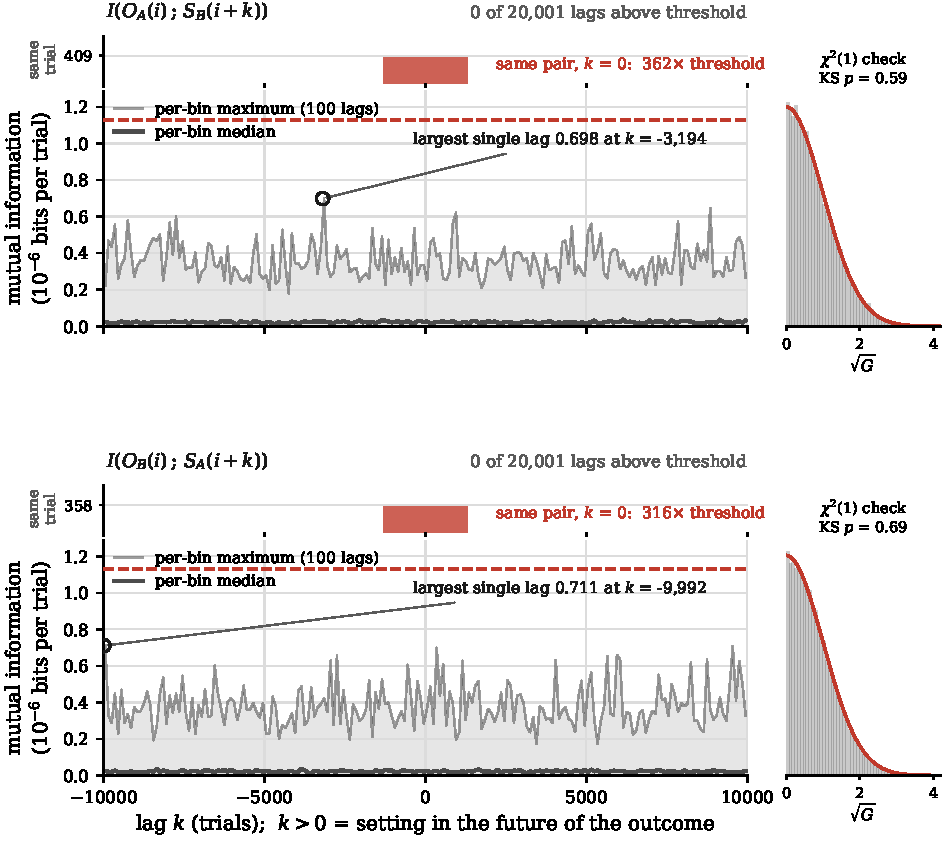
\includegraphics[width=\linewidth]{figures/fig1_mi_vs_lag.pdf}
\caption{Mutual information between one party's outcome at trial \textit{i} and the other party's setting at trial i+k, for all 20,001 lags $|k| \le 10{,}000$, round 28297. Both cross-pair channels are shown. The dashed line is the Bonferroni threshold at family-wise $\alpha$ = 0.05 over 40,002 hypotheses. The largest value in either channel reaches 63\% of the threshold. Vector version: \texttt{figures/fig1\_mi\_vs\_lag.pdf}.}
\label{fig:1}
\end{figure}

\subsection{The $J(k)$ curve}

The Eberhard statistic {[}9{]} for the CH-type inequality used by this
apparatus is

\begin{equation}
J \;=\; N(11|a_1b_1) - N(10|a_1b_2) - N(01|a_2b_1) - N(11|a_2b_2) \;\le\; 0
\label{eq:eberhard}
\end{equation}

under local realism, where \(N(o_A o_B \,|\, a\,b)\) counts trials with
the given settings and outcomes, and its uncertainty is the Poisson
propagation \(\sigma_J = \sqrt{N_1+N_2+N_3+N_4}\) over the four counts
entering J. Round 28297 gives J = 1,816 with \(\sigma_{\mathrm{J}}\) =
154.9, i.e.~\textbf{+11.7 (J/\(\sigma_{\mathrm{J}}\))}.

Computing the same statistic with settings from trial \emph{i} and
outcomes from trial i+k gives, for round 28297, +11.7 at \(k=0\) and a
mean of \(-135.5\) over the 106 nonzero lags (range \(-137.3\) to
\(-133.2\)) --- not merely consistent with zero, but far below the
violation boundary. Unlike the mutual-information scan of \S6.1, which
is exhaustive over all 20,001 lags, J(k) is evaluated at 107 sampled
lags: every lag from \(-50\) to +50, together with \(\pm 100,\)
\(\pm 1,000\) and \(\pm 10,000\) --- 106 nonzero lags plus the k = 0
control. The reason is cost, not principle: each J(k) requires a
separate pass over the full record, since the statistic has no FFT
shortcut, and as a sanity check rather than a bound it does not need
exhaustive coverage. The algebra is direct: when settings and outcomes
decouple, all four setting groups see the same outcome distribution, so
the two \(N(11|\cdot)\) terms cancel in expectation and the two
surviving single-click terms, which enter negatively, dominate. The
baseline level is pulse-dependent: across the ten pulses the least
negative nonzero lag ranges from \(-133.2\) (round 28297) to \(-168.6\)
(round 1000).

This is a sanity check, not a statistical test. By the identity of
Appendix C.2 the decoupled value of J is large and negative by
construction, so agreement with zero is not the question and no p-value
is attached to it. The question is whether J ever becomes
\emph{positive} --- whether a violation appears where none can exist.
Across all ten pulses, \(k \ne 0\) with \(J>0\): \textbf{0 of 1,060}
(106 nonzero lags \(\times\) 10 pulses). The peak falls from +11.7 to
the baseline within a single trial. There is no temporal tail. See
\textbf{Figure 2}.

\begin{figure}[htbp]
\centering
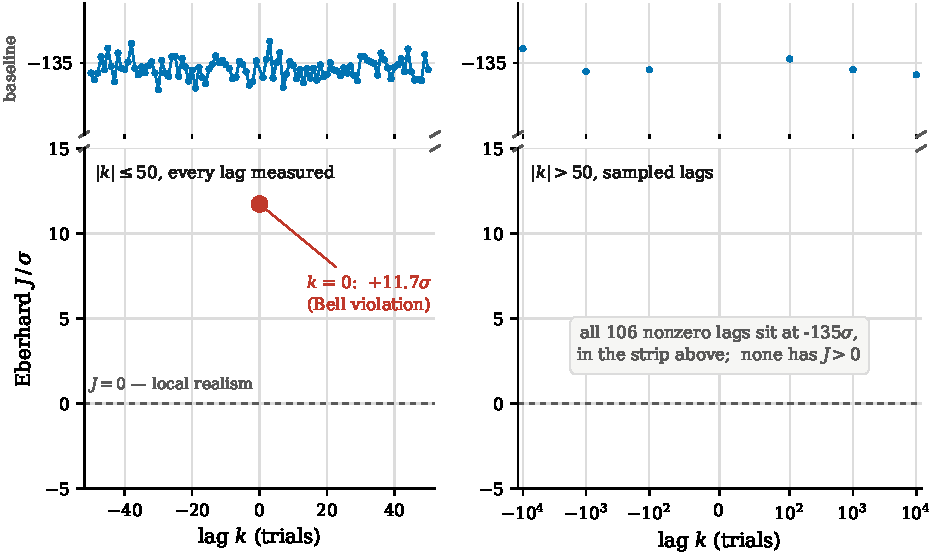
\includegraphics[width=\linewidth]{figures/fig2_j_curve.pdf}
\caption{Eberhard J in units of its Poisson error, as a function of the lag between settings and outcomes, round 28297. Left: |k| $\le$ 50, linear. Right: the full scanned range on a symmetric-log axis, showing that the behaviour at |k| up to 10,000 is identical to that at $|k| = 1$. The violation is confined to exactly one lag. Vector version: \texttt{figures/fig2\_j\_curve.pdf}.}
\label{fig:2}
\end{figure}

\subsection{Exclusion map}

The map of this section is not a second result. It is the bound of \S6.1
translated into the units of the model class of \S2: the same measured
click-rate differences \(\hat\delta(k)\), weighted by an assumed kernel
and converted to a coupling strength through the measured \(\alpha\).
Whatever one thinks of the kernels, the bits of \S6.1 stand on their
own; what the map adds is a reading of those bits in the language a
model would use.

\textbf{The statistic.} Let \(\hat\delta(k)\) be the estimator of
\(\delta(k)\) from the data: half the measured difference in click rate
between the two settings at lag k, computed from the \(2\times2\) table
at that lag. The optimal statistic is a matched filter on \(\hat\delta\)
rather than on \(\hat I\): \(\hat\delta\) is linear in the signal with
noise symmetric about zero, whereas \(\hat I\) is quadratic with
positive-definite noise that the filter would accumulate as bias. Define

\begin{equation}
T(\tau) \;=\; \sum_k W_\tau(k)\,\hat\delta(k), \qquad \mathbb{E}[T] = \alpha\,\varepsilon\,Q(\tau), \qquad \hat\varepsilon = \frac{T}{\alpha Q}, \qquad z = \frac{T}{\sigma_T}
\label{eq:T}
\end{equation}

Explicitly, \(\hat\varepsilon_A = T_A/(\alpha_A Q)\) for the pair
\(O_{\mathrm{A}}\) vs \(S_{\mathrm{B}}\), and
\(\hat\varepsilon_B = T_B/(\alpha_B Q)\) for \(O_{\mathrm{B}}\) vs
\(S_{\mathrm{A}}\): each channel is converted to a coupling strength
with the sensitivity of the party whose \emph{outcomes} are being
scanned --- \(\alpha_{\mathrm{A}}\) for Alice's outcomes, even though
the settings entering the filter are Bob's. Here \(\sigma_{\mathrm{T}}\)
is the standard deviation of T under the null. \(\sigma_{\mathrm{T}}\)
is obtained two ways and \textbf{the larger of the two is used}:
analytically,
\(\sigma_T = \sqrt{\textstyle\sum_k W(k)^2\sigma_\delta(k)^2}\) from the
binomial error of each \(2\times2\) table, and empirically, from 400
shuffles of the setting sequence per pair. The empirical and analytic
values agree to within 1.8\% on average per kernel (0.94--1.06 per
individual \(\tau\)). Two assumptions were verified rather than assumed:
the \(\hat\delta(k)\) are uncorrelated across k (\textbar r\textbar{}
\(\le\) 0.014 at \(\Delta k = 1, 2, 3, 5, 10\), against a standard error
of 0.007), and the null is centred (mean z under shuffling \(\le\) 0.05
in magnitude).

\textbf{Optimality, and what it assumes.} A matched filter is the
Neyman--Pearson optimal statistic for a signal of \emph{known shape} in
\emph{Gaussian white} noise. Both conditions are testable on these data
and both were tested. Whiteness is the uncorrelatedness of
\(\hat\delta(k)\) across k already quoted, \textbar r\textbar{} \(\le\)
0.014. Gaussianity: standardising each lag by its own binomial error,
the 20,001 values \(\hat\delta(k)/\sigma_\delta(k)\) have mean +0.0007
and standard deviation 0.9984 with a Kolmogorov--Smirnov p of 0.535 for
\(O_{\mathrm{A}}\) vs \(S_{\mathrm{B}}\), and mean +0.0062, standard
deviation 1.0000, p = 0.223 for \(O_{\mathrm{B}}\) vs
\(S_{\mathrm{A}}\). The tails, which are what a 4.85\(\sigma\) threshold
actually depends on, match too: 922 and 884 lags beyond 2\(\sigma\)
against 910 expected, 49 and 65 beyond 3\(\sigma\) against 54, none
beyond 4\(\sigma\) against 1.3 expected. Where the shape is \emph{not}
known --- the case the 1/\(\sqrt{Q}\) regularity below bears on ---
optimality is lost and the filter is merely valid: the threshold and the
bound remain correct, but some other filter could be more sensitive.

\textbf{Threshold.} The same \(z > 4.848\) as \S6.1 is used, i.e.~the
Bonferroni correction for 40,002 hypotheses is \emph{borrowed} for a
family of 208 tests. The matched correction for 208 tests would be
\(z > 3.672\); under it, every bound on the map would tighten by 16\% to
24\% (mean 22\%). The borrowed threshold is therefore deliberately
over-conservative by design, and keeps the map directly comparable with
the model-independent bound.

\textbf{Grid.} \(\tau\) takes 26 values:
\texttt{round(logspace(0, 4, 25))} together with 30 and 300, i.e.~1, 2,
3, 5, 7, 10, 15, 22, 30, 32, 46, 68, 100, 147, 215, 300, 316, 464, 681,
1000, 1468, 2154, 3162, 4642, 6813, 10000.

\(\varepsilon_{\mathrm{excl}}(\tau) = |\hat\varepsilon| + z_{\mathrm{thr}}\,\sigma_T/(\alpha Q)\),
for \(O_A\) vs \(S_B\):

\begin{longtable}[]{@{}
  >{\raggedright\arraybackslash}p{(\linewidth - 8\tabcolsep) * \real{0.2000}}
  >{\raggedright\arraybackslash}p{(\linewidth - 8\tabcolsep) * \real{0.2000}}
  >{\raggedright\arraybackslash}p{(\linewidth - 8\tabcolsep) * \real{0.2000}}
  >{\raggedright\arraybackslash}p{(\linewidth - 8\tabcolsep) * \real{0.2000}}
  >{\raggedright\arraybackslash}p{(\linewidth - 8\tabcolsep) * \real{0.2000}}@{}}
\caption{Excluded coupling strength
\(\varepsilon_{\mathrm{excl}}(\tau)\) for the four kernels,
\(O_{\mathrm{A}}\) vs \(S_{\mathrm{B}}\).}\tabularnewline
\toprule\noalign{}
\begin{minipage}[b]{\linewidth}\raggedright
\(\tau\) (trials)
\end{minipage} & \begin{minipage}[b]{\linewidth}\raggedright
symmetric
\end{minipage} & \begin{minipage}[b]{\linewidth}\raggedright
future-only
\end{minipage} & \begin{minipage}[b]{\linewidth}\raggedright
past-only
\end{minipage} & \begin{minipage}[b]{\linewidth}\raggedright
exp. future
\end{minipage} \\
\midrule\noalign{}
\endfirsthead
\toprule\noalign{}
\begin{minipage}[b]{\linewidth}\raggedright
\(\tau\) (trials)
\end{minipage} & \begin{minipage}[b]{\linewidth}\raggedright
symmetric
\end{minipage} & \begin{minipage}[b]{\linewidth}\raggedright
future-only
\end{minipage} & \begin{minipage}[b]{\linewidth}\raggedright
past-only
\end{minipage} & \begin{minipage}[b]{\linewidth}\raggedright
exp. future
\end{minipage} \\
\midrule\noalign{}
\endhead
\bottomrule\noalign{}
\endlastfoot
1 & \(7.559 \times 10^{-2}\) & \(9.954 \times 10^{-2}\) &
\(1.017 \times 10^{-1}\) & \(1.502 \times 10^{-1}\) \\
10 & \(1.533 \times 10^{-2}\) & \(1.949 \times 10^{-2}\) &
\(2.368 \times 10^{-2}\) & \(2.580 \times 10^{-2}\) \\
100 & \(4.277 \times 10^{-3}\) & \(6.207 \times 10^{-3}\) &
\(5.674 \times 10^{-3}\) & \(8.014 \times 10^{-3}\) \\
1,000 & \(1.493 \times 10^{-3}\) & \(2.023 \times 10^{-3}\) &
\(1.933 \times 10^{-3}\) & \(2.613 \times 10^{-3}\) \\
10,000 & \(4.373 \times 10^{-4}\) & \(6.407 \times 10^{-4}\) &
\(6.420 \times 10^{-4}\) & \(8.230 \times 10^{-4}\) \\
\end{longtable}

\textbf{Zero detections in 208 tests} (4 kernels \(\times\) 26 values of
\(\tau \times\) 2 pairs). Maximum \(|z| = 2.36\). The map is shown in
\textbf{Figure 3}.

\begin{figure}[htbp]
\centering
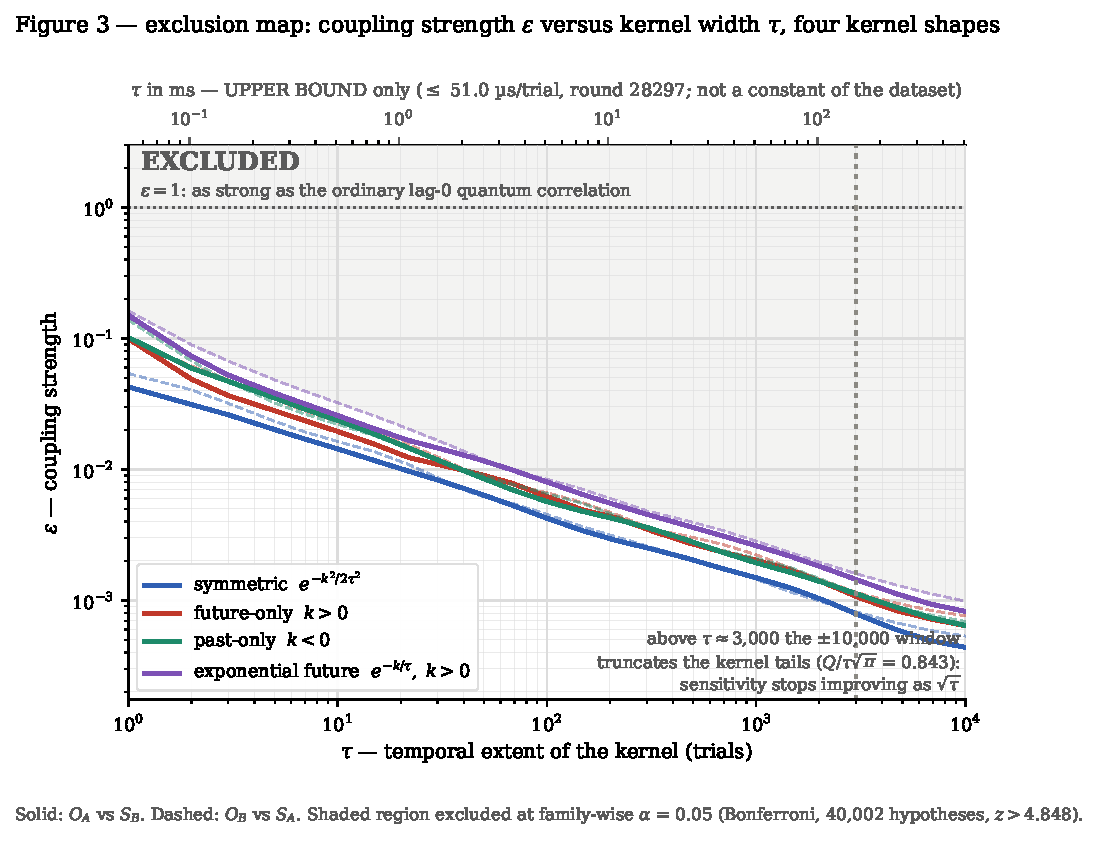
\includegraphics[width=\linewidth]{figures/fig3_exclusion_map.pdf}
\caption{Upper bound on the coupling strength $\varepsilon$ as a function of kernel width $\tau$, for all four kernel shapes and both cross-pair channels, round 28297. The shaded region is excluded at family-wise $\alpha$ = 0.05. The bend above $\tau \approx$ 3,000 is the finite scan window truncating the kernel tails. The upper axis gives the upper-bound conversion of \S4.1 and applies to this round only. Vector version: \texttt{figures/fig3\_exclusion\_map.pdf}.}
\label{fig:3}
\end{figure}

The one-sided bounds relax by the geometrically expected factor:
predicted \(\sqrt{2}\) = 1.414 against a measured median of 1.38 (range
1.18--1.56) for the one-sided Gaussians, and predicted
\(\sqrt{1/0.282}\) = 1.88 against a median of 1.85 (1.66--1.99) for the
exponential, over both pairs and \(\tau \ge\) 3. With k = 0 absent from
every kernel the expected factor is the same at all \(\tau\); the
scatter about it is the random data term \(|\hat\varepsilon|\), which is
largest at small \(\tau\), where each filter rests on a handful of lags.
These are factors of order unity, not orders of magnitude. The worst
value anywhere on the map is \(1.62 \times 10^{-1}\) --- even at its
weakest point, the analysis excludes coupling above one sixth of
ordinary quantum mechanics.

\textbf{Generalisation beyond the four shapes.} Since the noise on
\(\hat\delta(k)\) is approximately constant in k, the bound depends on
the kernel only through \(Q(\tau)=\sum_k W(k)^2\), and
\(\varepsilon_{\mathrm{excl}} \propto 1/\sqrt{Q}\). This was verified
numerically on the threshold term of the bound,
\(z_{\mathrm{thr}} \sigma_{\mathrm{T}}\)/(\(\alpha\)Q), which is the
part that carries the kernel dependence: its product with \(\sqrt{Q}\)
has a standard deviation of 3.5\% across all 208 points, most of which
is the difference between the two pairs (\(\alpha_A \ne \alpha_B\)),
with within-kernel scatter of about 2\%. The full product
\(\varepsilon_{\mathrm{excl}} \cdot \sqrt{Q}\) scatters more (8\%),
because it also contains the random data term \(|\hat\varepsilon|\) of
each kernel; the constant below is taken from the full product, so that
scatter is included in c.~The tested class is explicit: four families
\(\times\) 26 widths, 104 shapes, each measured in both channels. For
pre-specified kernels within the tested class, the observed sensitivity
follows an approximately universal 1/\(\sqrt{Q}\) scaling; the rigorous
exclusion is stated for the four explicit families. The table below
records that empirical regularity, tabulated by Q, and is offered as a
reading aid --- not as a theorem, and not as an exclusion of shapes that
were not tested:

\begin{longtable}[]{@{}
  >{\raggedright\arraybackslash}p{(\linewidth - 4\tabcolsep) * \real{0.3333}}
  >{\raggedright\arraybackslash}p{(\linewidth - 4\tabcolsep) * \real{0.3333}}
  >{\raggedright\arraybackslash}p{(\linewidth - 4\tabcolsep) * \real{0.3333}}@{}}
\caption{The empirical 1/\(\sqrt{Q}\) regularity of the bound within the
tested class, tabulated by Q. An empirical regularity, not a theorem;
the rigorous exclusion is the one stated for the four explicit
families.}\tabularnewline
\toprule\noalign{}
\begin{minipage}[b]{\linewidth}\raggedright
Q
\end{minipage} & \begin{minipage}[b]{\linewidth}\raggedright
\(\varepsilon_{\mathrm{excl}}\)
\end{minipage} & \begin{minipage}[b]{\linewidth}\raggedright
example shape
\end{minipage} \\
\midrule\noalign{}
\endfirsthead
\toprule\noalign{}
\begin{minipage}[b]{\linewidth}\raggedright
Q
\end{minipage} & \begin{minipage}[b]{\linewidth}\raggedright
\(\varepsilon_{\mathrm{excl}}\)
\end{minipage} & \begin{minipage}[b]{\linewidth}\raggedright
example shape
\end{minipage} \\
\midrule\noalign{}
\endhead
\bottomrule\noalign{}
\endlastfoot
3 & \(4.07 \times 10^{-2}\) & narrow kernel over \textasciitilde3
lags \\
10 & \(2.23 \times 10^{-2}\) & Gaussian \(\tau \approx\) 5.6,
exponential \(\tau \approx\) 20 \\
100 & \(7.05 \times 10^{-3}\) & Gaussian \(\tau \approx\) 56, square
over 100 lags \\
1,000 & \(2.23 \times 10^{-3}\) & Gaussian \(\tau \approx\) 564,
exponential \(\tau \approx\) 2,000 \\
10,000 & \(7.05 \times 10^{-4}\) & Gaussian \(\tau \approx\) 5,642 \\
\end{longtable}

with \(\varepsilon_{\mathrm{excl}}(Q)=c/\sqrt{Q}\), c = 0.0705 taken as
the maximum of \(\varepsilon\cdot\sqrt{Q}\) over the 168 points with
\(\tau \ge\) 10 (mean 0.0598), so that the table never promises a
tighter bound than was measured; checked against all four measured
kernels at \(\tau\) = 10, 100, 1,000 and 10,000, the formula is looser
than the measurement by factors of 1.03 to 1.32. Three conditions apply:
W normalised to max W = 1; summation within \(|k| \le 10{,}000\); and a
kernel specified in advance whose weight varies smoothly over its
support. The last condition is not decorative. The data term
\(|\hat\varepsilon|\) of each kernel is a random draw of the noise with
standard deviation 0.011/\(\sqrt{Q}\), of which c covers about 1.3
standard deviations on average --- ample for kernels that average over
many lags the way the four tested families do, but a kernel concentrated
on a few isolated lags can align with individual fluctuations of
\(\hat\delta(k)\) and exceed the tabulated value: an indicator kernel
placed on the three largest same-sign \(\hat\delta\) of this dataset
would need \(6.8 \times 10^{-2}\), 1.7 times the Q = 3 entry. Such
concentrated kernels --- and everything with Q \textless{} 3 --- should
be read against the measured \(\hat\delta(k)\) directly rather than from
the table.

This addresses the arbitrariness of the Gaussian choice only in part.
Within the tested class the sensitivity is set by Q and not by the
details of the shape, which is why the Gaussian was not a special
choice; but a kernel outside the tested class is not thereby excluded,
and no claim is made for it.

The map was verified by injection at four levels --- \(\varepsilon\) =
0, \(\varepsilon_{\mathrm{excl}}/2\), \(\varepsilon_{\mathrm{excl}}\)
and \(2\varepsilon_{\mathrm{excl}}\) --- with ten repetitions per point,
at two values of \(\tau\) for each of the three asymmetric kernels: six
points, sixty injections at each level. Detection is 0/60 at
\(\varepsilon\) = 0, 2/60 at half the bound, 39/60 at the bound and
60/60 at twice it, and the mean z scales linearly with \(\varepsilon\)
(\textbf{Figure 4}). The 39/60 at the bound itself is expected: a
confidence bound has by construction approximately 50\% power at the
bound, and quoting anything else would misrepresent it.

\begin{figure}[htbp]
\centering
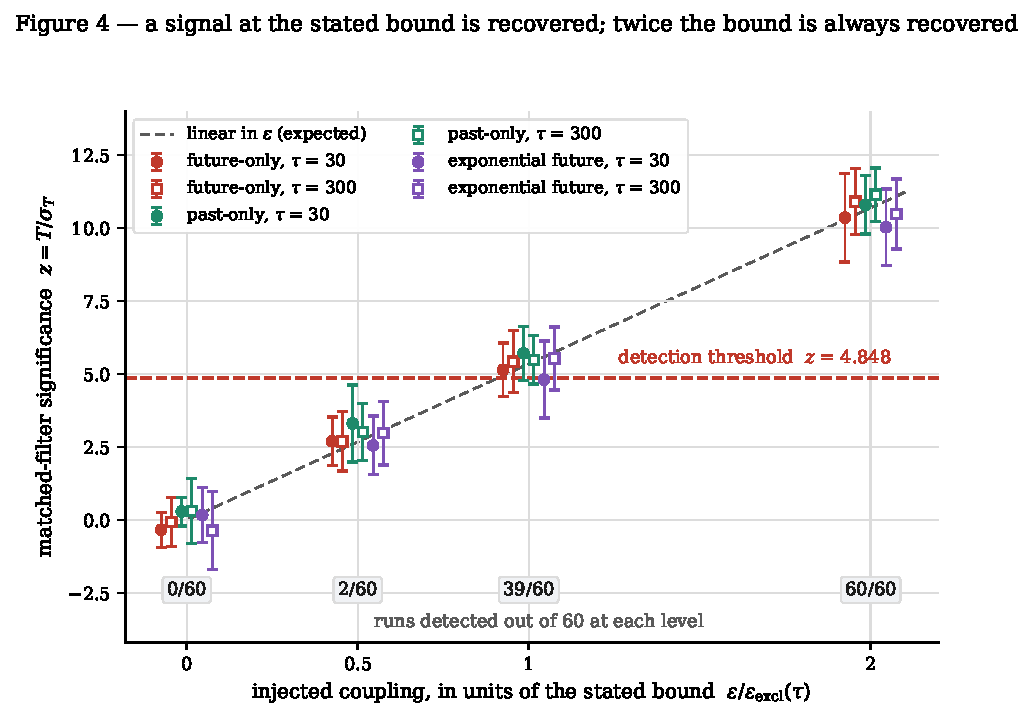
\includegraphics[width=\linewidth]{figures/fig4_injection_power.pdf}
\caption{Recovery of an injected signal of known strength. The horizontal axis is the injected coupling in units of the bound this analysis states for that kernel and $\tau$; the vertical axis is the matched-filter significance. Points are the mean over ten repetitions, error bars their standard deviation, and the six series are the three asymmetric kernels at $\tau$ = 30 and $\tau$ = 300. The dashed line is the linear scaling expected if the filter is unbiased. The boxes give the number of runs detected out of 60 at each level. Nothing is found when nothing is injected, and a signal at twice the stated bound is found every time. Vector version: \texttt{figures/fig4\_injection\_power.pdf}.}
\label{fig:4}
\end{figure}

\textbf{Kernel mismatch.} The mirror-filter test covers the extreme
case, a filter pointed the wrong way. The intermediate case is a filter
of the wrong \emph{width}. Injecting a symmetric Gaussian signal of
width \(\tau_{\mathrm{true}}\) and filtering it with a range of
\(\tau_{\mathrm{filter}}\) gives, as a fraction of the matched value:

\begin{longtable}[]{@{}
  >{\raggedright\arraybackslash}p{(\linewidth - 18\tabcolsep) * \real{0.1000}}
  >{\raggedright\arraybackslash}p{(\linewidth - 18\tabcolsep) * \real{0.1000}}
  >{\raggedright\arraybackslash}p{(\linewidth - 18\tabcolsep) * \real{0.1000}}
  >{\raggedright\arraybackslash}p{(\linewidth - 18\tabcolsep) * \real{0.1000}}
  >{\raggedright\arraybackslash}p{(\linewidth - 18\tabcolsep) * \real{0.1000}}
  >{\raggedright\arraybackslash}p{(\linewidth - 18\tabcolsep) * \real{0.1000}}
  >{\raggedright\arraybackslash}p{(\linewidth - 18\tabcolsep) * \real{0.1000}}
  >{\raggedright\arraybackslash}p{(\linewidth - 18\tabcolsep) * \real{0.1000}}
  >{\raggedright\arraybackslash}p{(\linewidth - 18\tabcolsep) * \real{0.1000}}
  >{\raggedright\arraybackslash}p{(\linewidth - 18\tabcolsep) * \real{0.1000}}@{}}
\caption{Loss of significance when the filter width does not match the
signal width, measured over five injections at
\(4\varepsilon_{\mathrm{excl}}\) and compared with the closed form
\(\sum_k W_f(k)W_t(k)\big/\sqrt{\sum_k W_f(k)^2 \cdot \sum_k W_t(k)^2}\),
which is 1 when the widths match. The last column departs from the
closed form at \(\tau_{\mathrm{true}} = 3{,}000\) because the
\(\pm 10,000\) window truncates a filter of width
30,000.}\tabularnewline
\toprule\noalign{}
\begin{minipage}[b]{\linewidth}\raggedright
\(\tau_{\mathrm{filter}}/\tau_{\mathrm{true}}\)
\end{minipage} & \begin{minipage}[b]{\linewidth}\raggedright
0.1
\end{minipage} & \begin{minipage}[b]{\linewidth}\raggedright
1/3
\end{minipage} & \begin{minipage}[b]{\linewidth}\raggedright
0.5
\end{minipage} & \begin{minipage}[b]{\linewidth}\raggedright
0.825
\end{minipage} & \begin{minipage}[b]{\linewidth}\raggedright
1
\end{minipage} & \begin{minipage}[b]{\linewidth}\raggedright
1.21
\end{minipage} & \begin{minipage}[b]{\linewidth}\raggedright
2
\end{minipage} & \begin{minipage}[b]{\linewidth}\raggedright
3
\end{minipage} & \begin{minipage}[b]{\linewidth}\raggedright
10
\end{minipage} \\
\midrule\noalign{}
\endfirsthead
\toprule\noalign{}
\begin{minipage}[b]{\linewidth}\raggedright
\(\tau_{\mathrm{filter}}/\tau_{\mathrm{true}}\)
\end{minipage} & \begin{minipage}[b]{\linewidth}\raggedright
0.1
\end{minipage} & \begin{minipage}[b]{\linewidth}\raggedright
1/3
\end{minipage} & \begin{minipage}[b]{\linewidth}\raggedright
0.5
\end{minipage} & \begin{minipage}[b]{\linewidth}\raggedright
0.825
\end{minipage} & \begin{minipage}[b]{\linewidth}\raggedright
1
\end{minipage} & \begin{minipage}[b]{\linewidth}\raggedright
1.21
\end{minipage} & \begin{minipage}[b]{\linewidth}\raggedright
2
\end{minipage} & \begin{minipage}[b]{\linewidth}\raggedright
3
\end{minipage} & \begin{minipage}[b]{\linewidth}\raggedright
10
\end{minipage} \\
\midrule\noalign{}
\endhead
\bottomrule\noalign{}
\endlastfoot
\(\tau_{\mathrm{true}} = 30\) & 0.425 & 0.777 & 0.897 & 0.990 & 1 &
0.993 & 0.904 & 0.784 & 0.440 \\
\(\tau_{\mathrm{true}} = 300\) & 0.434 & 0.794 & 0.909 & 0.995 & 1 &
0.987 & 0.882 & 0.758 & 0.425 \\
\(\tau_{\mathrm{true}} = 3{,}000\) & 0.433 & 0.769 & 0.887 & 0.989 & 1 &
0.992 & 0.903 & 0.822 & 0.734 \\
closed form & 0.444 & 0.774 & 0.894 & 0.991 & 1 & 0.991 & 0.894 & 0.774
& 0.445 \\
\end{longtable}

The \(\tau\) grid is logarithmic with step \(10^{4/24} = 1.468\), so a
signal falling exactly between two grid points is mismatched by a factor
1.212 --- and loses \textbf{0.9\%} of z. The grid is dense enough that
nothing can hide between its points. Even gross misspecification
degrades gracefully: a factor of two costs 10\%, a factor of three 22\%,
a factor of ten 56\%. The filter is never blind, only less sensitive.

Measured z initially exceeded prediction by 3--7\%. The cause is not
physical: the map uses \(\sigma_{\mathrm{T}}\) = max(empirical,
analytic) whereas the verification computes z from the analytic value
alone. With 400 shuffles the empirical estimate carries \(\pm 3.5\)\%
noise, and the max() systematically selects upward fluctuations. The
measured ratio \(z_{\mathrm{obs}}/z_{\mathrm{pred}} = 1.035\) decomposes
as \(\sigma_T(\mathrm{map})/\sigma_T(\mathrm{analytic}) = 1.018\) times
a residual of 1.016 \(\pm\) 0.015, consistent with unity. Doubling the
shuffle count from 400 to 800 moves the ratio from 1.046 to 1.007 as
expected for an estimation artefact. An alternative mechanism ---
reduced autocorrelation in injected data --- was tested and excluded:
the outcome autocorrelation is zero at every lag from 1 to 5 (maximum
\textbar r\textbar{} = \(3.1 \times 10^{-4}\) against a standard error
of \(2.6 \times 10^{-4}\)), and \(\sigma_{\mathrm{T}}\) computed from
shuffles of injected versus real data agrees to within error with the
sign varying between cases.

Sensitivity ceases to improve as \(\sqrt\tau\) above \(\tau \approx\)
3,000, where the \(\pm 10,000\) scan window begins truncating the kernel
tails (\(Q(10^4)/\tau\sqrt{\pi} = 0.843\)). This is visible as a bend in
Figure 3 and is not smoothed.

\subsection{Joint bound from the ten pulses}

The map above uses one pulse. The other nine can be combined with it,
but not by concatenation: they are separated by months, the click rate
falls by a third across them, and \(\alpha\) varies by 20\% (Limitation
1). Splicing them into a single sequence would create an object with no
physical counterpart and would import the drift as spurious structure.

Each pulse is therefore analysed on its own terms --- its own
\(\hat\delta(k)\), its own \(\sigma_{\mathrm{T}}\) from 400 shuffles of
its own setting sequence, its own \(\alpha\) --- and the resulting
estimates are combined with inverse-variance weights:

\begin{equation}
\hat\varepsilon_{\mathrm{joint}} = \frac{\sum_p \hat\varepsilon_p/\sigma_p^2}{\sum_p 1/\sigma_p^2}, \qquad \sigma_{\mathrm{joint}} = \Big(\sum_p 1/\sigma_p^2\Big)^{-1/2}
\label{eq:joint}
\end{equation}

with \(\hat\varepsilon_p = T_p/(\alpha_p Q)\) and
\(\sigma_p = \sigma_{T,p}/(\alpha_p Q)\), and the joint bound formed as
before,
\(|\hat\varepsilon_{\mathrm{joint}}| + z_{\mathrm{thr}}\sigma_{\mathrm{joint}}\).
A pulse with small \(\alpha\) has large \(\sigma_{\mathrm{p}}\) and
contributes less: sensitivity sets the weight, not trial count.

\begin{longtable}[]{@{}
  >{\raggedright\arraybackslash}p{(\linewidth - 10\tabcolsep) * \real{0.1667}}
  >{\raggedright\arraybackslash}p{(\linewidth - 10\tabcolsep) * \real{0.1667}}
  >{\raggedright\arraybackslash}p{(\linewidth - 10\tabcolsep) * \real{0.1667}}
  >{\raggedright\arraybackslash}p{(\linewidth - 10\tabcolsep) * \real{0.1667}}
  >{\raggedright\arraybackslash}p{(\linewidth - 10\tabcolsep) * \real{0.1667}}
  >{\raggedright\arraybackslash}p{(\linewidth - 10\tabcolsep) * \real{0.1667}}@{}}
\caption{Joint exclusion from all ten pulses, \(O_{\mathrm{A}}\) vs
\(S_{\mathrm{B}}\), with the improvement over the single-pulse map of
\S6.3.}\tabularnewline
\toprule\noalign{}
\begin{minipage}[b]{\linewidth}\raggedright
\(\tau\) (trials)
\end{minipage} & \begin{minipage}[b]{\linewidth}\raggedright
symmetric
\end{minipage} & \begin{minipage}[b]{\linewidth}\raggedright
future-only
\end{minipage} & \begin{minipage}[b]{\linewidth}\raggedright
past-only
\end{minipage} & \begin{minipage}[b]{\linewidth}\raggedright
exp. future
\end{minipage} & \begin{minipage}[b]{\linewidth}\raggedright
gain over \S6.3
\end{minipage} \\
\midrule\noalign{}
\endfirsthead
\toprule\noalign{}
\begin{minipage}[b]{\linewidth}\raggedright
\(\tau\) (trials)
\end{minipage} & \begin{minipage}[b]{\linewidth}\raggedright
symmetric
\end{minipage} & \begin{minipage}[b]{\linewidth}\raggedright
future-only
\end{minipage} & \begin{minipage}[b]{\linewidth}\raggedright
past-only
\end{minipage} & \begin{minipage}[b]{\linewidth}\raggedright
exp. future
\end{minipage} & \begin{minipage}[b]{\linewidth}\raggedright
gain over \S6.3
\end{minipage} \\
\midrule\noalign{}
\endhead
\bottomrule\noalign{}
\endlastfoot
1 & \(1.945 \times 10^{-2}\) & \(2.655 \times 10^{-2}\) &
\(2.564 \times 10^{-2}\) & \(4.345 \times 10^{-2}\) & 3.4--3.8 \\
10 & \(3.564 \times 10^{-3}\) & \(5.898 \times 10^{-3}\) &
\(5.783 \times 10^{-3}\) & \(8.380 \times 10^{-3}\) & 3.1--4.4 \\
100 & \(1.145 \times 10^{-3}\) & \(1.625 \times 10^{-3}\) &
\(1.653 \times 10^{-3}\) & \(2.339 \times 10^{-3}\) & 3.4--3.8 \\
1,000 & \(3.523 \times 10^{-4}\) & \(4.976 \times 10^{-4}\) &
\(4.940 \times 10^{-4}\) & \(7.077 \times 10^{-4}\) & 3.8--4.3 \\
10,000 & \(1.234 \times 10^{-4}\) & \(2.089 \times 10^{-4}\) &
\(2.188 \times 10^{-4}\) & \(2.770 \times 10^{-4}\) & 3.0--3.6 \\
\end{longtable}

\textbf{Zero detections in 208 joint tests}, maximum
\(|z_{\mathrm{joint}}| = 2.10\). The mean improvement over the
single-pulse map is a factor \textbf{3.62} (range 2.77 to 5.10), which
exceeds the naive \(\sqrt{10} = 3.16\) for the reason given in
Limitation 1: round 28297 has the third-smallest \(\alpha\) of the ten,
within 2\% of the smallest, so the comparison is against one of the
least sensitive pulses. The gain column is computed against the
independent re-estimate of the 28297 map described below, so that both
sides of the ratio carry the same shuffle noise; dividing the printed
tables instead reproduces it to within the \(\pm 3.5\)\% noise of the
empirical \(\sigma_{\mathrm{T}}\). The worst joint bound anywhere on the
map is \(4.34 \times 10^{-2}\), against \(1.62 \times 10^{-1}\) for the
single pulse.

As a by-product this run re-estimates the 28297 map independently, with
a different shuffle seed; it reproduces the published values of \S6.3
with a mean ratio of 1.005 and a range of 0.95 to 1.08, consistent with
the \(\pm 3.5\)\% estimation noise on the empirical
\(\sigma_{\mathrm{T}}\) discussed above.

\textbf{Independence of the pulses.} Inverse-variance weighting is
optimal, and \(\sigma_{\mathrm{joint}}\) is correct, only if the ten
estimates are uncorrelated. Five of the pulses (28293--28297) were
acquired consecutively within 65 minutes, so this cannot be assumed.
Since \(T_{\mathrm{p}}\) is a linear functional of the \(\hat\delta(k)\)
of pulse p, any covariance between pulses would have to appear as a
correlation between the \(\hat\delta(k)\) of one pulse and the
\(\hat\delta(k)\) of another across lags. This was measured directly:
for each of the 45 pairs of pulses and each channel, the Pearson
correlation of the standardised \(\hat\delta(k)/\sigma_\delta(k)\) of
one pulse with that of the other over the 20,000 lags k \(\ne\) 0, whose
standard error under independence is 1/\(\sqrt{20}\),000 = 0.0071. The
largest \textbar r\textbar{} among the 90 values is 0.018
(2.6\(\sigma\), pulses 23000 and 28293, which are three months apart);
among the twenty values from the five consecutive pulses the largest is
0.015 (2.1\(\sigma\), pulses 28294 and 28295), and the mean is
\(-0.002.\) The standard deviation of r across pairs is 0.0072 and
0.0077 in the two channels, against 0.0071 expected, and no pair exceeds
3\(\sigma\). The pulses are uncorrelated at the level the data can
resolve, and the diagonal covariance assumed by the weights is measured
rather than assumed. Had a substantial correlation appeared, the
combination would have required generalised least squares with the full
covariance matrix; it does not.

That test is at the level of the lags. The quantity the joint bound
actually depends on is the covariance of the estimators
\(T_{\mathrm{p}}\) themselves, and covariance concentrated in the few
lags where a narrow kernel puts its weight would move an unweighted
correlation over 20,000 lags very little while still biasing
\(\sigma_{\mathrm{joint}}\). It was therefore computed directly, for
each of the 104 filters, each of the 45 pulse pairs and both channels.
Since \(T_p = \sum_k W(k)\,\hat\delta_p(k)\) and the \(\hat\delta\) are
uncorrelated across k, the covariance is
\(\sum_k W(k)^2 \mathrm{Cov}(\hat\delta_p, \hat\delta_q)\), whose
estimator standardised by its own sampling error is
\(t_{pq} = \sum_k W(k)^2 z_p z_q / \sqrt{\sum_k W(k)^4}\) with
\(z = \hat\delta/\sigma_\delta\), standard normal if the pulses are
independent. A \(W^{2}\)-weighted \emph{correlation} would be the wrong
statistic and would saturate at \(\pm 1\): the effective number of lags
a filter uses, \((\sum W^2)^2/\sum W^4\), is 1.1 for the future kernel
at \(\tau\) = 1. Across the 9,360 values of t the mean is +0.029 and the
standard deviation 0.955 against 0 and 1, and the largest is 4.18 where
4.28 is expected as the maximum of that many normals. Keeping the
measured off-diagonal terms would move \(\sigma_{\mathrm{joint}}\) by
+1.3\% on average over the filters that rest on ten or more lags;
against a null built by giving each pulse an independent random circular
shift of its lag axis, which destroys any alignment between pulses while
preserving each pulse's own structure, that shift is +0.58\(\sigma\),
and the corresponding figure over all filters is +0.86\(\sigma\). There
is no covariance beyond what independent pulses produce, and the
diagonal weighting stands.

The combination also assumes a coupling common to the ten pulses --- not
a triviality across twenty-two months of drifting hardware. The
assumption was tested rather than left implicit: for each kernel and
\(\tau\), the heterogeneity statistic
\(Q_{\mathrm{het}} = \sum_p (\hat\varepsilon_p - \hat\varepsilon_{\mathrm{joint}})^2/\sigma_p^2\)
follows \(\chi^{2}\)(9) if one \(\varepsilon\) underlies all ten pulses.
Over the 208 points of the map its mean is 8.0 against the expected 9.0
--- mildly under-dispersed, the signature of the conservative
\(\sigma_{\mathrm{T}}\) = max(empirical, analytic) --- and the largest
value, 28.5, has a family-corrected p of 0.17 across the 208 strongly
correlated points. The ten pulses are statistically consistent with a
single coupling, here zero. If the coupling nevertheless varied across
epochs, the joint bound would constrain its inverse-variance-weighted
mean, and the per-pulse maps (\S6.3, Limitation 1) remain the
epoch-resolved statements.

The joint bound is the strongest statement this dataset supports. The
single-pulse map of \S6.3 is retained as the quoted result elsewhere in
this paper because \S6.1, \S6.2, \S6.5 and the injection verification
are all single-pulse and are directly comparable with it.

\subsection{Outcome--outcome correlation}

If the trial sequence were temporally scrambled --- Alice's and Bob's
records mispaired --- the signature would appear not in outcome--setting
but in outcome--outcome correlation. Scanning I(\(O_{\mathrm{A}}\)(i) ;
\(O_{\mathrm{B}}\)(i+k)):

\begin{longtable}[]{@{}
  >{\raggedright\arraybackslash}p{(\linewidth - 2\tabcolsep) * \real{0.5000}}
  >{\raggedright\arraybackslash}p{(\linewidth - 2\tabcolsep) * \real{0.5000}}@{}}
\caption{Outcome--outcome scan, round 28297.}\tabularnewline
\toprule\noalign{}
\endfirsthead
\endhead
\bottomrule\noalign{}
\endlastfoot
k = 0 (positive control) & \(1.4267 \times 10^{-2}\) bits, G = 296,670
(545\(\sigma\) on the \(\sqrt{G}\) scale) \\
max at k \(\ne\) 0 & \(7.3232 \times 10^{-7}\) bits, at lag
\(-2,526\) \\
above threshold & 0 / 20,000 \\
\end{longtable}

\begin{equation}
\boxed{\;I\big(O_A(i) ; O_B(i+k)\big) \;<\; 1.066\times10^{-6}\ \text{bits per trial}\quad\text{for every } 0 < |k| \le 10{,}000\;}
\label{eq:bound2}
\end{equation}

This test involves a single pair rather than two, so the Bonferroni
family is 20,001 hypotheses rather than 40,002 and the threshold is
correspondingly lower, \(1.066 \times 10^{-6}\) instead of
\(1.130 \times 10^{-6}\). The count ``0 / 20,000'' excludes k = 0, which
is the positive control and is expected to exceed the threshold --- the
20,001st hypothesis is the control itself.

The bound is 1/13,384 of the Bell correlation at k = 0. Detector
deadtime does not appear here either (G \(\le\) 1.61, i.e.~\(\le\)
1.3\(\sigma\), at \(|k| \le 2\)).

Repeated identically on all ten pulses, the scan gives \textbf{0 of
200,000} nonzero lags above threshold, the largest value being
4.4\(\sigma\); the k = 0 control lies between 508\(\sigma\) and
552\(\sigma\) in every pulse, and the coincidence enhancement over
independent outcomes grows from 38\(\times\) (round 1000) to
59\(\times\) (the 2025 pulses) as the click rate falls.

\subsection{Single-party memory}

The scans above are cross-party: one party's outcome against the
\emph{other} party's setting. Memory of a device's \emph{own} settings
--- I(\(O_{\mathrm{A}}\)(i) ; \(S_{\mathrm{A}}\)(i+k)) at k \(\ne\) 0
--- is a distinct channel. It cannot fake a Bell violation by itself,
but it is the natural signature of a stateful detector or setting
generator, and until now it had been examined only at \(|k| = 1\), as
the deadtime entry of \S5, on one pulse. The same 20,001-lag scan as
\S6.1 --- same \(\chi^2(1)\) machinery, same threshold --- was therefore
run on both same-party channels, \(O_{\mathrm{A}}\) vs
\(S_{\mathrm{A}}\) and \(O_{\mathrm{B}}\) vs \(S_{\mathrm{B}}\), in all
ten pulses. The lag k = 0 is the positive control: it carries the
ordinary same-trial setting dependence that this analysis calibrates
against (\(\sqrt{G}\) between 85.8 and 139.5 across the twenty channels)
and is excluded from the count.

\textbf{Zero detections in 400,000 tests} (20,000 nonzero lags
\(\times\) 2 channels \(\times\) 10 pulses). The largest value anywhere
is \(\sqrt{G}\) = 4.82, at lag \(-5,819\) of round 1000
(\(O_{\mathrm{B}}\) vs \(S_{\mathrm{B}}\)), reaching 98.8\% of the
threshold --- and this is what the null predicts for a family of this
size: the expected number of \(\chi^2(1)\) draws above that point in
400,000 tests is 0.58. Neither device retains a measurable memory of its
own settings at any lag the window reaches, in any pulse.

\subsection{Parity of setting pairs}

Every test so far is marginal in the settings: it asks whether the
outcome depends on \emph{one} setting at \emph{one} lag. A dependence on
a joint function of several settings whose single-setting marginals
vanish --- the simplest being the parity of two adjacent settings ---
would be invisible to all of it. The parity of a balanced independent
pair is itself a balanced binary sequence, so the identical machinery
applies: define P(i) = 1 if S(i) = S(i+1), and scan
I(\(O_{\mathrm{A}}\)(i) ; \(P_{\mathrm{B}}\)(i+k)) and
I(\(O_{\mathrm{B}}\)(i) ; \(P_{\mathrm{A}}\)(i+k)) over all 20,001 lags,
in all ten pulses, at the same threshold. No lag is a positive control
here: the parity is independent of each single setting by construction,
so even k = 0 must be null. The \(\chi^2(1)\) calibration was
re-verified on the parity sequence directly (mean G = 1.025 over 200
shuffles).

\textbf{Zero detections in 400,020 tests} (20,001 lags \(\times\) 2
channels \(\times\) 10 pulses). The largest value anywhere is
\(\sqrt{G}\) = 4.50, at lag \(-1,777\) of round 28297, reaching 86\% of
the threshold. The outcomes depend on no adjacent-pair parity anywhere
in the window. This closes the quadratic-adjacent case only; functionals
of three or more settings, and of non-adjacent pairs, remain untested
(Limitation 7).

\textbf{Relevance to device-independent protocols.} Device-independent
randomness generation and device-independent quantum key distribution
rest on the assumption that the devices carry no exploitable memory
between trials --- that the statistics of trial i are not conditioned on
the settings of other trials. That assumption is exactly the memory
loophole {[}10{]}, and it is the reason such protocols are analysed with
adversarially valid, memory-tolerant statistics {[}11--13{]} rather than
with the i.i.d. estimates that would otherwise suffice. Dropping the
assumption costs more than a looser bound: Weilenmann, Budroni and
Navascués {[}27{]} show that in the non-i.i.d. regime whole classes of
certification become impossible, membership tests for non-convex sets of
correlations among them, so how well the assumption holds decides what
can be certified at all. The results of this paper --- 0 of 400,000
single-party memory tests (\S6.6), 0 of 200,010 setting-correlation
tests (\S5.1), and the bound of \(1.13 \times 10^{-6}\) bits per trial
on the information any outcome carries about any other trial's setting
(\S6.1) --- constitute a direct empirical check of that assumption on an
operating beacon, and the check is independent of any interpretation of
the model class of \S2. It does not establish the security of the
protocol: what is verified is one assumption, at the stated sensitivity,
on these records.

\subsection{Oscillatory kernels: a frequency scan}

All four kernel families of \S2.2 are one-signed, and an oscillatory
coupling is nearly orthogonal to every one of them: it would pass the
matched filters of \S6.3 unseen. It is also the shape with the most
mundane possible origin --- mains pickup, a modulation of the pump, any
periodic drive in the apparatus --- which makes it worth testing rather
than conceding.

\textbf{The statistic.} A Lomb--Scargle periodogram of the standardised
\(\hat\delta(k)/\sigma_\delta(k)\) over the 20,000 lags k \(\ne\) 0.
Lomb--Scargle rather than a plain periodogram because the lag grid is
uniform apart from the single missing point at k = 0, which it handles
exactly instead of by interpolation. In the Scargle normalisation the
power at each frequency is Exp(1) under Gaussian white noise, and both
conditions were established in \S6.3: the \(\hat\delta(k)\) are
uncorrelated across k (\textbar r\textbar{} \(\le\) 0.014) and Gaussian
(Kolmogorov--Smirnov p = 0.535 and 0.223). The frequency grid is
\(f_j = j/20{,}001\) cycles per lag for j = 1 \ldots{} 10,000, so M =
10,000 searched frequencies per channel, and the Bonferroni threshold on
Exp(1) is \(z = \ln(m/0.05)\): z = 12.90 for the two channels of one
pulse (m = 20,000) and z = 15.20 for the ten pulses (m = 200,000), the
latter matching the family construction of \S6.5, \S6.6 and \S6.7.
Frequencies are reported in cycles per lag; the conversion to Hz is
nominal, through the \textasciitilde4 \(\mu\)s per trial of \S4.1, and
the metadata upper bound of 51 \(\mu\)s per trial would divide every
frequency by 12.7.

\textbf{Round 28297.} In \(O_{\mathrm{A}}\) vs \(S_{\mathrm{B}}\) the
largest power is 9.02, at a period of 2.4 lags, against an expected null
maximum of \(\ln M + \gamma = 9.79\): nothing. In \(O_{\mathrm{B}}\) vs
\(S_{\mathrm{A}}\) the largest power is 13.38, at f = 0.00330 cycles per
lag, a period of 303 lags --- 825 Hz on the nominal conversion, 65 Hz on
the metadata bound, neither of which is a mains harmonic. That value
sits just above the single-pulse threshold, at 104\% of it, and below
the ten-pulse threshold. Its probability within one channel is
\(1-(1-e^{-P})^M = 0.015\), so roughly 0.03 across the two channels of
the pulse: a one-in-thirty fluctuation, which is what a threshold set at
\(\alpha\) = 0.05 is built to admit. The mean power is 1.0000 in both
channels, exactly the Exp(1) expectation, and the frequency nearest 50
Hz nominal carries power 1.20 and 0.78.

\textbf{It does not repeat.} A periodic drive in the apparatus would
appear in more than one record, and above all in the five pulses taken
consecutively within 65 minutes of one day. The other nine pulses were
therefore scanned in full, both channels, and the 303-lag frequency
examined in each. No channel of any of them has a maximum above even the
single-pulse threshold --- the largest anywhere is 12.22 --- so
\textbf{no frequency in the ten pulses reaches the ten-pulse threshold:
0 of 200,000}. At the 303-lag frequency itself the power across the
other eighteen pulse-channels has mean 1.12 and maximum 3.86, an
unremarkable Exp(1) sample; in the other channel of round 28297 it is
0.53. The excess is confined to one channel of one pulse and is
consistent with noise. It is reported rather than dropped, and the
ten-pulse scan is reported as what it is: a follow-up run after the
single-pulse scan produced it, not an independent pre-specified test.

\textbf{Sensitivity and control.} A sinusoid of amplitude A in white
noise of width \(\sigma\) carries Lomb--Scargle power
\(\approx N A^2/4\sigma^2\), so the threshold corresponds to a coupling
\(\varepsilon_{\mathrm{thr}} = \sqrt{4z/N}\,\sigma_\delta/\alpha = 5.5\times10^{-4}\)
for an oscillatory kernel of unit peak --- comparable to the
\(\varepsilon_{\mathrm{excl}}\) the one-signed kernels reach near
\(\tau \approx 10^{3}\), and the number that now replaces the untested
caveat of Limitation 2. The machinery was verified by injecting an
oscillatory coupling at the outcome level,
\(\lambda(i) = \lambda_0 + \alpha\varepsilon \sum_{k \neq 0} \cos(2\pi f_0 k + \varphi)\, S_B(i+k)\),
with a fresh random phase each repetition: at 2\(\varepsilon\)\_thr the
peak is found, and found at \(f_{0}\), in 5 of 5 repetitions at periods
of 7, 137 and 5,000 lags, and at \(\varepsilon_{\mathrm{thr}}\) in about
half, as a confidence bound requires. The analytic threshold was also
checked against 400 permutations of the lag ordering: their maxima have
mean 9.81 and 95th percentile 12.06, and 2.2\% exceed z = 12.90, against
the 2.5\% per channel that Bonferroni promises.

\section{Limitations}

\begin{enumerate}
\def\labelenumi{\arabic{enumi}.}
\tightlist
\item
  The exclusion map of \S6.3 derives from one pulse (28297); the joint
  bound of \S6.4 uses all ten, as do the setting-correlation test of
  \S5.1 and the single-party memory scan of \S6.6, the parity scan of
  \S6.7, and the outcome--outcome scan of \S6.5. The injection
  verification (Figure 4) was run on 28297 alone. \(\alpha\) varies
  across the archive by 20\% (standard deviation, against 0.94\%
  measurement error per pulse), tracking the falling click rate. Round
  28297 has the third-smallest \(\alpha\) of the ten --- only rounds
  28293 and 28294 lie lower, by 0.8\% and 1.6\% --- and since
  \(\varepsilon_{\mathrm{excl}} \propto 1/\alpha\) the single-pulse map
  is within 2\% of the loosest that any of the ten would yield: at equal
  n, another pulse would give a bound 0.60\(\times\) to 1.02\(\times\)
  the stated value. That restriction is therefore conservative to within
  2\% rather than merely unquantified, and it is why the joint
  improvement exceeds \(\sqrt{10}\).
\item
  Oscillatory kernels are covered only in part. The map of \S6.3 does
  not reach them at all: its 1/\(\sqrt{Q}\) regularity is empirical and
  established only within the tested class of one-signed kernels, and an
  oscillatory kernel has a different optimal filter shape entirely.
  \S6.8 covers the \emph{purely sinusoidal} case, where all the power
  sits at one frequency, and bounds such a coupling of unit peak at
  \(\varepsilon\) \textless{} \(5.5 \times 10^{-4}\) across all ten
  pulses. It does \emph{not} fully cover a modulated or damped
  oscillation --- a decaying sinusoid, or one whose amplitude varies
  over its support --- because an envelope spreads the power over a band
  of frequencies, so no single periodogram bin carries the whole signal
  and the sensitivity degrades by roughly the number of bins the power
  is spread across. Between the two lies the same gap as before: a
  kernel that is neither one-signed nor a single sinusoid is constrained
  by neither statistic at full sensitivity.
\item
  The injection places the coupling in one channel. A model acting
  coherently in both was not tested.
\item
  Lags \(|k| > 10{,}000\) and widths \(\tau\) \textgreater{} 10,000 were
  not examined; the window already constrains sensitivity above
  \(\tau \approx\) 3,000.
\item
  Time and calibration are confounded across the spread pulses; a
  difference could not be attributed to either. The conversion from
  trials to seconds is an upper bound and is not constant across the
  archive (\S4.1).
\item
  Measurement independence is bounded, not excluded. Models below
  threshold remain viable, and within-trial retrocausality is entirely
  untouched.
\item
  The bounds concern dependence of an outcome on a single setting
  (\S6.1--6.6) or on the parity of two adjacent settings (\S6.7),
  matching the model class of \S2, which is linear in the settings.
  Dependence on functionals of three or more settings, or of
  non-adjacent pairs, with vanishing lower-order marginals is not
  constrained.
\end{enumerate}

\section{Conclusion}

Across ten pulses of a loophole-free Bell test spanning twenty-two
months, no correlation was found between measurement outcomes and
settings chosen at any other trial. The statement to carry away is the
model-independent one: I(O ; S at lag k) \textless{}
\(1.13 \times 10^{-6}\) bits per trial for every lag up to
\(\pm 10,000,\) at family-wise \(\alpha\) = 0.05 --- 1/362 of the
same-trial correlation the same instrument registers --- while the
outcome--outcome information at nonzero lag stays below 1/13,384 of the
Bell correlation, and no outcome lets any other trial's setting be
guessed with a bias above \(1.25 \times 10^{-3}\) (\S6.1). The
instrument is not insensitive.

Translated into the parameters of the model class of \S2, the same data
exclude \(\varepsilon\) above \(7.6 \times 10^{-2}\) at \(\tau\) = 1 and
\(4.4 \times 10^{-4}\) at \(\tau\) = \(10^{4}\) on a single pulse,
across four kernel shapes including the future-directed ones natural to
retrocausal models. That map is the bits above re-expressed in model
units, not a second result; within the tested class the sensitivity
follows an approximately universal 1/\(\sqrt{Q}\) scaling, and the
rigorous exclusion is stated for the four explicit families. Combining
the ten pulses by weight, with the pulses shown to be uncorrelated, the
excluded coupling falls to \(1.9 \times 10^{-2}\) and
\(1.2 \times 10^{-4}\) at the same two widths, and the weakest point of
the entire joint map --- the narrowest kernel, \(\tau\) = 1 --- still
excludes \(\varepsilon\) above \(4.34 \times 10^{-2}\). The same holds
within each wing separately --- neither device shows any correlation
with its own settings at nonzero lag, in any of the ten pulses (\S6.6)
--- and for the simplest joint functional of the settings, the parity of
adjacent pairs (\S6.7). A frequency scan of all ten pulses adds the one
shape the matched filters cannot see, an oscillatory kernel, and finds
nothing above threshold in 200,000 frequencies (\S6.8).

What would a nonzero \(\varepsilon\) have implied, and what does its
absence buy? Within the model class every kernel excludes k = 0 (\S2.2)
and so never touches the same-trial statistic; cross-trial coupling of
any strength cannot by itself fake the observed Bell violation ---
Figure 2 shows this directly. Its operational cost lies elsewhere: in
the assumption, made whenever such records certify randomness, that
trials do not leak information about one another. That leakage is what
the bound prices --- less than \(1.13 \times 10^{-6}\) bits per trial
about any single setting up to ten thousand trials away, or a guessing
bias below \(1.25 \times 10^{-3}\). The bound cannot be converted into a
bound on Hall's \(I(X,Y:\Lambda)\); the data-processing inequality runs
the wrong way (\S1). What is constrained is the operationally effective
part of measurement dependence, not the hidden variable itself --- the
strongest statement data of this kind permit, and the weakest a skeptic
must grant.

This does not refute retrocausal models; the class they occupy is
within-trial and is not addressed here. What it does is convert an
untested assumption into a measured constraint --- including the
no-memory assumption on which device-independent randomness and DI-QKD
rest, verified here on an operating beacon at the stated sensitivity,
without a claim of security. The region is now mapped.

\clearpage
\appendix
\section{Which script produces which number}

\begin{longtable}[]{@{}
  >{\raggedright\arraybackslash}p{(\linewidth - 2\tabcolsep) * \real{0.5000}}
  >{\raggedright\arraybackslash}p{(\linewidth - 2\tabcolsep) * \real{0.5000}}@{}}
\caption{Which script produces which number.}\tabularnewline
\toprule\noalign{}
\begin{minipage}[b]{\linewidth}\raggedright
Script
\end{minipage} & \begin{minipage}[b]{\linewidth}\raggedright
Produces
\end{minipage} \\
\midrule\noalign{}
\endfirsthead
\toprule\noalign{}
\begin{minipage}[b]{\linewidth}\raggedright
Script
\end{minipage} & \begin{minipage}[b]{\linewidth}\raggedright
Produces
\end{minipage} \\
\midrule\noalign{}
\endhead
\bottomrule\noalign{}
\endlastfoot
\texttt{code/katevasma.py}, \texttt{code/load\_curby.py} & download and
unpack the beacon records; SHA-256 manifest \\
\texttt{code/xartografisi.py} & \S4: protocol parameters of 25 rounds
(\texttt{results/xartografisi\_cache.json}) \\
\texttt{code/full\_scan.py} & \S6.1: 20,001-lag scan, \(\chi^2(1)\)
calibration, thresholds, Figure 1 data \\
\texttt{code/j\_curve.py} & \S6.2: J(k), the shift-sign self-test,
Figure 2 data \\
\texttt{code/stability10.py} & \S6.2: the ten-pulse J values and the
0-of-1,060 count \\
\texttt{code/lag\_dense.py}, \texttt{code/lag\_test.py} & the 111-lag
scans of Limitation 1; the deadtime entry of \S5 \\
\texttt{code/meros1\_alpha.py} & \S3: \(r_{1}\), \(r_{2}\),
\(\delta\)(0), \(\alpha\), C, exact vs approximate I \\
\texttt{code/meros2\_injection.py} & \S3: injection test of the analytic
relation, clipping \\
\texttt{code/meros3\_map.py}, \texttt{code/meros3\_verify.py} & \S6.3:
matched filter, symmetric map, injection verification \\
\texttt{code/meros4\_outcome\_outcome.py} & \S6.5: outcome--outcome scan
and k = 0 control \\
\texttt{code/meros5\_asym.py}, \texttt{code/meros5\_verify.py} & \S6.3:
the four kernels, mirror-filter test \\
\texttt{code/meros6\_p0.py} & \S3: \(p_{0}\) as marginal, exact MI, the
\(2.2 \times 10^{-16}\) reconstruction \\
\texttt{code/meros6\_systematic.py} & \S6.3: decomposition of the 3--7\%
systematic \\
\texttt{code/meros6\_kernelQ.py} & \S6.3: \(\varepsilon \propto\)
1/\(\sqrt{Q}\) and the Q \(\rightarrow \varepsilon_{\mathrm{excl}}\)
table \\
\texttt{code/meros6\_alpha10.py} & Limitation 1: \(\alpha\) for each of
the ten pulses \\
\texttt{code/meros7\_power.py} & \S6.3: the \(\varepsilon\) = 0 and
\(\varepsilon_{\mathrm{excl}}/2\) levels of Figure 4 \\
\texttt{code/meros8\_settings.py} & \S5.1: setting correlations and the
phantom signal \\
\texttt{code/meros9\_joint.py} & \S6.4: per-pulse analysis and the
inverse-variance joint bound \\
\texttt{code/meros10\_settings10.py} & \S5.1: the phantom check across
all ten pulses \\
\texttt{code/meros11\_optimality.py} & \S6.3: Gaussianity of
\(\hat\delta\), kernel-mismatch loss \\
\texttt{code/meros12\_selfmemory.py} & \S6.6: single-party memory scan,
all ten pulses \\
\texttt{code/meros13\_parity.py} & \S6.7: setting-pair parity scan, all
ten pulses \\
\texttt{code/meros14\_oo10.py} & \S6.5: the ten-pulse outcome--outcome
scan \\
\texttt{code/meros15\_homogeneity.py} & \S6.4:
\(\varepsilon\)-homogeneity test; \S6.3: matched-threshold factors \\
\texttt{code/meros16\_crosspulse.py} & \S6.4: cross-pulse correlation of
\(\hat\delta(k)\), the pulse-independence row of Table 3 \\
\texttt{code/meros17\_periodogram.py} & \S6.8: Lomb--Scargle periodogram
of \(\hat\delta(k)\), its threshold, null and positive control \\
\texttt{code/meros18\_covariance.py} & \S6.4: covariance of the
\(T_{\mathrm{p}}\) across pulses, per filter, and its permutation
null \\
\texttt{code/check\_refs.py} & verifies every internal cross-reference
resolves \\
\texttt{code/figures\_en.py} & Figures 1--3 \\
\end{longtable}

\section{Reproduction}

\begin{verbatim}
python3 code/katevasma.py --rounds 28297
python3 code/load_curby.py curby_round_28297.bin --out curby_28297.npz
python3 code/full_scan.py ; python3 code/meros1_alpha.py
python3 code/meros2_injection.py ; python3 code/meros3_map.py
python3 code/meros3_verify.py ; python3 code/meros4_outcome_outcome.py
python3 code/meros5_asym.py ; python3 code/meros5_verify.py
python3 code/meros6_p0.py ; python3 code/meros6_kernelQ.py
python3 code/meros6_systematic.py ; python3 code/meros6_alpha10.py
python3 code/meros7_power.py ; python3 code/meros8_settings.py
python3 code/meros9_joint.py ; python3 code/meros10_settings10.py
python3 code/meros11_optimality.py ; python3 code/meros12_selfmemory.py
python3 code/meros13_parity.py ; python3 code/meros14_oo10.py
python3 code/meros15_homogeneity.py ; python3 code/meros16_crosspulse.py
python3 code/meros17_periodogram.py ; python3 code/meros18_covariance.py
python3 code/figures_en.py
\end{verbatim}

Random seeds are fixed in the scripts: 4711 (exclusion map shuffles),
808 and 909 (injection verification), 1707 (power curve), 2026
(systematic diagnostics), 3141 (mismatch), 5150 (joint bound), 0 and
\textbar k\textbar+1 (per-lag nulls). Results were produced with Python
3.14.6, NumPy 2.5.1, SciPy 1.18.0 and Matplotlib 3.11.1; the minimum
supported versions are given in \texttt{requirements.txt}.

\section{Derivations}

\subsection{Second-order expansion of the mutual information}

Let the setting take two values with equal probability, and write
\(r_{1}\), \(r_{2}\) for the conditional click rates, \(p_{0}\) =
\((r_1+r_2)/2\) for the marginal, and \(\delta\) =
(\(r_{2} - r_{1}\))/2. The mutual information of the \(2\times2\) table
is

\begin{equation}
I \;=\; \sum_{s,o} P(s,o)\,\log_2\!\left[\frac{P(s,o)}{P(s)P(o)}\right]
\label{eq:mi-def}
\end{equation}

With \(P(s) = \tfrac12\) and \(r_{1,2} = p_0 \mp \delta\), expanding
each term to second order in \(\delta/p_0\) and \(\delta/(1-p_0)\):

\begin{equation}
P(o{=}1|s)\,\log_2\!\left[\frac{P(o{=}1|s)}{p_0}\right] \;=\; (p_0 \pm \delta)\log_2\!\left(1 \pm \frac{\delta}{p_0}\right) \;=\; \frac{\pm\delta + \delta^2/2p_0}{\ln 2} + O(\delta^3)
\label{eq:expansion}
\end{equation}

and similarly for o=0 with \(p_0 \to 1-p_0\). Averaging over the two
settings, the first-order terms cancel by construction, leaving

\begin{equation}
I \;=\; \frac{1}{\ln 2}\left[\frac{\delta^2}{2p_0} + \frac{\delta^2}{2(1-p_0)}\right] \;=\; \frac{\delta^2}{2\ln 2\; p_0(1-p_0)} + O(\delta^3)
\label{eq:expansion2}
\end{equation}

The expansion parameter is \(\delta\)/\(p_{0}\), not \(p_{0}\) itself;
for the present data \(\delta/p_0 = 0.283\) and the residual is 1.35\%,
in the direction of underestimating I. The exact four-term sum is used
wherever precision matters; the expansion serves only to exhibit the
\(\varepsilon^{2}\) scaling and to define C.

\subsection{The Eberhard statistic at nonzero lag}

Write the Eberhard {[}9{]} combination as

\begin{equation}
J \;=\; N(o{=}11\,|\,a_1b_1) - N(o{=}10\,|\,a_1b_2) - N(o{=}01\,|\,a_2b_1) - N(o{=}11\,|\,a_2b_2)
\label{eq:eberhard2}
\end{equation}

where \(N(\cdot|\cdot)\) counts trials with the indicated outcome pair
and setting pair, and \(J \le 0\) for any local hidden-variable model.

When outcomes are taken from trial \(i+k\) with \(k \ne 0\) while
settings are taken from trial i, the two are statistically independent.
Each of the four setting groups then sees the same outcome distribution,
and with \(n/4\) trials per group and outcome probabilities
\(P_{11}, P_{10}, P_{01}\) for the joint outcomes:

\begin{equation}
J \;\to\; \frac{n}{4}\left[P_{11} - P_{10} - P_{01} - P_{11}\right] \;=\; -\frac{n}{4}\left(P_{10} + P_{01}\right)
\label{eq:eberhard-lag}
\end{equation}

The two \(P_{11}\) terms enter with opposite sign and cancel exactly.
What survives is minus the exclusive single-click rate, and one subtlety
fixes its size: the two outcomes at trial i+k are taken as a \emph{pair}
from a single trial, so their joint distribution retains the full Bell
correlation of the source. For round 28297 the coincidence rate is
\(P_{11}\) = \(2.79 \times 10^{-3}\) --- 59 times the
\(4.8 \times 10^{-5}\) that independent outcomes would give --- and the
exclusive singles are \(P_{10}\) = \(4.14 \times 10^{-3}\) and
\(P_{01}\) = \(4.08 \times 10^{-3}\). The identity then predicts J =
\(-30,800\) and, from the Poisson propagation over the four counts,
\(\sigma_{\mathrm{J}}\) = 227, hence J/\(\sigma_{\mathrm{J}}\) =
\(-135.6\) --- against the observed mean of \(-135.5\) (\S6.2). The
decoupled value of J is therefore large and negative rather than near
zero, and the observed level is reproduced quantitatively by the
identity alone. The relevant test is not whether \(J\) is small at
\(k \ne 0\) but whether it is ever positive; across ten pulses and 106
nonzero lags each, it is not.

\section*{Data and code availability}

Analysis code, intermediate results, and figures are available at
\url{https://github.com/christosgeorgitzikis47/cross-trial-bell-bound}.
Raw data are public at random.colorado.edu; per-round URLs and SHA-256
digests are listed in \texttt{results/curby\_manifest.json}.

\section*{Acknowledgements}

I thank Krister Shalm (NIST) for directing me to the raw trial records
and for answering an unsolicited enquiry from an independent researcher.

\begin{thebibliography}{9}
\bibitem{r1} B. Hensen et al., \textit{Nature} \textbf{526}, 682 (2015).
\bibitem{r2} L. K. Shalm et al., \textit{Phys. Rev. Lett.} \textbf{115}, 250402 (2015).
\bibitem{r3} G. A. Kavuri et al., ``Traceable random numbers from a non-local quantum advantage'', \textit{Nature} (2025), DOI 10.1038/s41586-025-09054-3.
\bibitem{r4} M. J. W. Hall, \textit{Phys. Rev. Lett.} \textbf{105}, 250404 (2010).
\bibitem{r5} H. Price, \textit{Time's Arrow and Archimedes' Point}, Oxford University Press (1996).
\bibitem{r6} K. B. Wharton and N. Argaman, ``Colloquium: Bell's theorem and locally mediated reformulations of quantum mechanics'', \textit{Rev. Mod. Phys.} \textbf{92}, 021002 (2020).
\bibitem{r7} M. S. Leifer and M. F. Pusey, \textit{Proc. R. Soc. A} \textbf{473}, 20160607 (2017).
\bibitem{r8} R. Chaves et al., ``Causal networks and freedom of choice in Bell's theorem'', arXiv:2105.05721 (2021).
\bibitem{r9} P. H. Eberhard, \textit{Phys. Rev. A} \textbf{47}, R747 (1993).
\bibitem{r10} J. Barrett, D. Collins, L. Hardy, A. Kent, S. Popescu, \textit{Phys. Rev. A} \textbf{66}, 042111 (2002).
\bibitem{r11} R. D. Gill, ``Accardi contra Bell (cum mundi): the impossible coupling'', in \textit{Mathematical Statistics and Applications: Festschrift for Constance van Eeden}, IMS Lecture Notes --- Monograph Series \textbf{42}, 133 (2003).
\bibitem{r12} Y. Zhang, S. Glancy, E. Knill, \textit{Phys. Rev. A} \textbf{84}, 062118 (2011).
\bibitem{r13} P. Bierhorst, \textit{J. Phys. A} \textbf{48}, 195302 (2015).
\bibitem{r14} J. E. Pope, A. Kay, \textit{Phys. Rev. A} \textbf{88}, 032110 (2013).
\bibitem{r15} G. Pütz, D. Rosset, T. J. Barnea, Y.-C. Liang, N. Gisin, \textit{Phys. Rev. Lett.} \textbf{113}, 190402 (2014).
\bibitem{r16} D. Aktas et al., \textit{Phys. Rev. Lett.} \textbf{114}, 220404 (2015).
\bibitem{r17} J. Handsteiner et al., \textit{Phys. Rev. Lett.} \textbf{118}, 060401 (2017).
\bibitem{r18} D. Rauch et al., \textit{Phys. Rev. Lett.} \textbf{121}, 080403 (2018).
\bibitem{r19} J. Barrett, R. Colbeck, A. Kent, \textit{Phys. Rev. Lett.} \textbf{110}, 010503 (2013).
\bibitem{r20} K. B. Wharton, ``A novel interpretation of the Klein-Gordon equation'', \textit{Found. Phys.} \textbf{40}, 313 (2010), arXiv:0706.4075.
\bibitem{r21} K. B. Wharton, ``Time-symmetric boundary conditions and quantum foundations'', \textit{Symmetry} \textbf{2}, 272 (2010).
\bibitem{r22} J. Barrett, N. Gisin, ``How much measurement independence is needed in order to demonstrate nonlocality?'', \textit{Phys. Rev. Lett.} \textbf{106}, 100406 (2011), arXiv:1008.3612.
\bibitem{r23} M. J. W. Hall, C. Branciard, ``Measurement-dependence cost for Bell nonlocality: Causal versus retrocausal models'', \textit{Phys. Rev. A} \textbf{102}, 052228 (2020), arXiv:2007.11903.
\bibitem{r24} D. E. Koh, M. J. W. Hall, Setiawan, J. E. Pope, C. Marletto, A. Kay, V. Scarani, A. Ekert, ``Effects of reduced measurement independence on Bell-based randomness expansion'', \textit{Phys. Rev. Lett.} \textbf{109}, 160404 (2012), arXiv:1202.3571.
\bibitem{r25} J.-Å. Larsson, ``Loopholes in Bell inequality tests of local realism'', \textit{J. Phys. A: Math. Theor.} \textbf{47}, 424003 (2014).
\bibitem{r26} E. Santos, ``On possible memory effects in tests of Bell inequalities'', arXiv:1603.04428 (2016).
\bibitem{r27} M. Weilenmann, C. Budroni, M. Navascués, ``Memory attacks in network nonlocality and self-testing'', \textit{Quantum} \textbf{9}, 1735 (2025).
\end{thebibliography}

\end{document}
